% A LaTeX template for MSc Thesis submissions to 
% Politecnico di Milano (PoliMi) - School of Industrial and Information Engineering
%
% S. Bonetti, A. Gruttadauria, G. Mescolini, A. Zingaro
% e-mail: template-tesi-ingind@polimi.it
%
% Last Revision: October 2021
%
% Copyright 2021 Politecnico di Milano, Italy. NC-BY

\documentclass[bibliography=numbered]{Configuration_Files/PoliMi3i_thesis}

%------------------------------------------------------------------------------
%	REQUIRED PACKAGES AND  CONFIGURATIONS
%------------------------------------------------------------------------------

% CONFIGURATIONS
\usepackage{parskip} % For paragraph layout
\usepackage{setspace} % For using single or double spacing
\usepackage{emptypage} % To insert empty pages
\usepackage{multicol} % To write in multiple columns (executive summary)
\setlength\columnsep{15pt} % Column separation in executive summary
\setlength\parindent{0pt} % Indentation
\raggedbottom  

% PACKAGES FOR TITLES
\usepackage{titlesec}
% \titlespacing{\section}{left spacing}{before spacing}{after spacing}
\titlespacing{\section}{0pt}{3.3ex}{2ex}
\titlespacing{\subsection}{0pt}{3.3ex}{1.65ex}
\titlespacing{\subsubsection}{0pt}{3.3ex}{1ex}
\usepackage{color}

% PACKAGES FOR LANGUAGE AND FONT
\usepackage[english]{babel} % The document is in English  
\usepackage[utf8]{inputenc} % UTF8 encoding
\usepackage[T1]{fontenc} % Font encoding
\usepackage[11pt]{moresize} % Big fonts

% PACKAGES FOR IMAGES
\usepackage{graphicx}
\usepackage{transparent} % Enables transparent images
\usepackage{eso-pic} % For the background picture on the title page
\usepackage{subfig} % Numbered and caption subfigures using \subfloat.
\usepackage{tikz} % A package for high-quality hand-made figures.
\usetikzlibrary{}
\graphicspath{{./Images/}} % Directory of the images
\usepackage{caption} % Coloured captions
\usepackage{xcolor} % Coloured captions
\usepackage{amsthm,thmtools,xcolor} % Coloured "Theorem"
\usepackage{float}

% STANDARD MATH PACKAGES
\usepackage{amsmath}
\usepackage{amsthm}
\usepackage{amssymb}
\usepackage{amsfonts}
\usepackage{bm}
\usepackage[overload]{empheq} % For braced-style systems of equations.
\usepackage{fix-cm} % To override original LaTeX restrictions on sizes

% PACKAGES FOR TABLES
\usepackage{tabularx}
\usepackage{longtable} % Tables that can span several pages
\usepackage{colortbl}
\usepackage{multicol}

% PACKAGES FOR ALGORITHMS (PSEUDO-CODE)
\usepackage{algorithm}
\usepackage{algorithmic}
\usepackage{listings}

% PACKAGES FOR REFERENCES & BIBLIOGRAPHY
\usepackage[colorlinks=true,linkcolor=black,anchorcolor=black,citecolor=black,filecolor=black,menucolor=black,runcolor=black,urlcolor=black]{hyperref} % Adds clickable links at references
%\usepackage{cleveref}
\usepackage{babel}
\usepackage[maxcitenames=2, 
  maxbibnames=99, 
  backend=biber, 
  citestyle=authoryear, 
  bibstyle=authoryear, 
  sorting=nyt, %sort by name title year 
  natbib=true,
  giveninits=true,
  hyperref
  ]{biblatex} % CustomBib
%\usepackage[square, numbers, sort&compress]{natbib} % Square brackets, citing references with numbers, citations sorted by appearance in the text and compressed
%\bibliographystyle{abbrvnat} % You may use a different style adapted to your field

% OTHER PACKAGES
\usepackage{pdfpages} % To include a pdf file
\usepackage{afterpage}
\usepackage{lipsum} % DUMMY PACKAGE
\usepackage{fancyhdr} % For the headers
\fancyhf{}
\usepackage{wrapfig}

% MY PACKAGES
\usepackage{changepage}
% Input of configuration file. Do not change config.tex file unless you really know what you are doing. 
% Define blue color typical of polimi
\definecolor{bluepoli}{cmyk}{0.4,0.1,0,0.4}

% Custom theorem environments
\declaretheoremstyle[
  headfont=\color{bluepoli}\normalfont\bfseries,
  bodyfont=\color{black}\normalfont\itshape,
]{colored}

% Set-up caption colors
\captionsetup[figure]{labelfont={color=bluepoli}} % Set colour of the captions
\captionsetup[table]{labelfont={color=bluepoli}} % Set colour of the captions
\captionsetup[algorithm]{labelfont={color=bluepoli}} % Set colour of the captions

\theoremstyle{colored}
\newtheorem{theorem}{Theorem}[chapter]
\newtheorem{proposition}{Proposition}[chapter]

% Enhances the features of the standard "table" and "tabular" environments.
\newcommand\T{\rule{0pt}{2.6ex}}
\newcommand\B{\rule[-1.2ex]{0pt}{0pt}}

% Pseudo-code algorithm descriptions.
\newcounter{algsubstate}
\renewcommand{\thealgsubstate}{\alph{algsubstate}}
\newenvironment{algsubstates}
  {\setcounter{algsubstate}{0}%
   \renewcommand{\STATE}{%
     \stepcounter{algsubstate}%
     \Statex {\small\thealgsubstate:}\space}}
  {}

% New font size
\newcommand\numfontsize{\@setfontsize\Huge{200}{60}}

% Title format: chapter
\titleformat{\chapter}[hang]{
\fontsize{50}{20}\selectfont\bfseries\filright}{\textcolor{bluepoli} \thechapter\hsp\hspace{2mm}\textcolor{bluepoli}{|   }\hsp}{0pt}{\huge\bfseries \textcolor{bluepoli}
}

% Title format: section
\titleformat{\section}
{\color{bluepoli}\normalfont\Large\bfseries}
{\color{bluepoli}\thesection.}{1em}{}

% Title format: subsection
\titleformat{\subsection}
{\color{bluepoli}\normalfont\large\bfseries}
{\color{bluepoli}\thesubsection.}{1em}{}

% Title format: subsubsection
\titleformat{\subsubsection}
{\color{bluepoli}\normalfont\large\bfseries}
{\color{bluepoli}\thesubsubsection.}{1em}{}

% Shortening for setting no horizontal-spacing
\newcommand{\hsp}{\hspace{0pt}}

\makeatletter
% Renewcommand: cleardoublepage including the background pic
\renewcommand*\cleardoublepage{%
  \clearpage\if@twoside\ifodd\c@page\else
  \null
  \AddToShipoutPicture*{\BackgroundPic}
  \thispagestyle{empty}%
  \newpage
  \if@twocolumn\hbox{}\newpage\fi\fi\fi}
\makeatother

%For correctly numbering algorithms
\numberwithin{algorithm}{chapter}
%----------------------------------------------------------------------------
%	NEW COMMANDS DEFINED
%----------------------------------------------------------------------------

\newcommand{\bea}{\begin{eqnarray}} % Shortcut for equation arrays
\newcommand{\eea}{\end{eqnarray}}
\newcommand{\e}[1]{\times 10^{#1}}  % Powers of 10 notation
\bibliography{bibliography.bib}
%----------------------------------------------------------------------------
%	BEGIN OF YOUR DOCUMENT
%----------------------------------------------------------------------------

\begin{document}

\fancypagestyle{plain}{%
\fancyhf{} % Clear all header and footer fields
\fancyhead[RO,RE]{\thepage} %RO=right odd, RE=right even
\renewcommand{\headrulewidth}{0pt}
\renewcommand{\footrulewidth}{0pt}}

%----------------------------------------------------------------------------
%	TITLE PAGE
%----------------------------------------------------------------------------

\pagestyle{empty} % No page numbers
\frontmatter % Use roman page numbering style (i, ii, iii, iv...) for the preamble pages

\puttitle{
	title=eMall -- e-Mobility for all,
	nameA=Fabio Lusha - 10882532,
	nameB=Bianca C. Savoiu Marinas - 10684465,
	academicyear=2022-2023
}
\startpreamble
\setcounter{page}{1} % Set page counter to 1

%----------------------------------------------------------------------------
%	LIST OF CONTENTS/FIGURES/TABLES/SYMBOLS
%----------------------------------------------------------------------------

% TABLE OF CONTENTS
\thispagestyle{empty}
\tableofcontents % Table of contents 
\thispagestyle{empty}
\cleardoublepage

\addtocontents{toc}{\vspace{2em}} % Add a gap in the Contents, for aesthetics
\mainmatter % Begin numeric (1,2,3...) page numbering

% ----------------------
% CHAPTERS
% ----------------------

\chapter{Introduction}
\label{ch:chapter_one}%
\section{Purpose}
\label{sec:purpose}%
Widespread electrification of transport is the most efficient way to reach Europe’s climate objectives for the sector and electric charging is the main asset to overcome the obstacles of the take-up of electric vehicles (EVs). EVs can reduce CO2 by an estimated annual 600,000 tons by 2030, going towards a carbon neutral Europe, and the importance of this aim raises the problem of having efficient systems that manage the charging services. The eMall is thought as an all-encompassing application that oversees the entire process from the user interaction to the effective recharge of the EV's battery.

The main goal we want to achieve with the eMall software is to help The EVDs (electric vehicle drivers) to have a better access to recharge and to be able to book a charging point in order to avoid interference with his daily plans. Another important purpose of the system is to safeguard not only the users but also the providers of the service and this is made through privacy agreements and the actual interaction, that guarantees to supervise both interested parts, in order to get the best possible service and pay for it accordingly, having also a technical and economic exploitation of the charging infrastructures.

In this context there is an increase in the requested electric energy, but large amounts of power in short periods would require investments in the reinforcement of the distribution networks, which have not been designed to accommodate such load. It becomes necessary to introduce new systems and solutions to optimize the operation of the distribution networks. In this context we can identify the DSOs as the suppliers of electricity through the distribution networks. The DSOs interact with the eMall, and in particular with the CPMS (Charging Point Management System) module of the system to be. The CPMS, then, gives the information about the DSO's supply to the CPOs, which are important actors, that use the system in order to manage the charging service. A CPO is represented by an employee or a software, part of the business that owns some charging stations and wants to manage them through the eMall, deciding from where to acquire energy, and how to establish the prices, the special offers and other details about the stations.

The eMall is thought as a software that manages both the interaction with the businesses that offer the charging service and the interaction with the EVDs which want to use these services in order to charge their EVs. Therefore, the eMall provides a mobile application (eMma), which through its interface allows to the EVD to obtain the service, and provides, also, a web application that the CPOs use to manage the charging stations. The EVD interacts, as well, with the charging point interface (eMci), that communicates with the CPMS part of the eMall, in order to start the charging session from the station, plugging then the car to the compatible connector to effectively charge the EV.

\paragraph{Goals} In the following table we present the main goals of the software to be. The goals capture the needs of the stakeholders, which are the EVDs and the CPOs.

\newcounter{gc}
\setcounter{gc}{1}
\newcommand{\gcnt}{\thegc\stepcounter{gc}}
\begin{table}[H]
    \centering
    \begin{tabular}{|l|p{0.9\linewidth}|}
     \hline
     \textbf{Goal} & \textbf{Description} \\
     \hline
     G\gcnt & The EVD is able to identify the charging stations nearby \\
     \hline
     G\gcnt & The EVD is able to visualize the tariffs of the charging stations \\
     \hline
     G\gcnt & The EVD is able to visualize any special offer available at the charging station \\
     \hline
     G\gcnt & The EVD is able to book a charge in a specific charging station for a certain time frame\\
     \hline
     G\gcnt & The EVD is able to start the charging process at a certain station \\
     \hline
     G\gcnt & The EVD is able to pay for the obtained service \\
     \hline
     G\gcnt & The CPO can decide from which DSO to acquire energy \\
     \hline 
     G\gcnt & The CPO can decide the cost of charging \\
     \hline 
     G\gcnt & The CPO can set special offers \\
     \hline 
     G\gcnt & The CPO can decide whether to store or not energy in batteries \\
     \hline 
     G\gcnt & The CPO can decide whether to use the energy available in the batteries \\
     \hline 
\end{tabular}
    \caption{Goals}
    \label{tab:Goals}
\end{table}

\section{Scope}
\label{sec:Scope}%
\paragraph{World phenomena} The portion of the real world where the machine is to be deployed and used is called the environment. Hence, scoping the problem by defining the environment is paramount, and this is the target of the next table. With the world phenomena we define the environment in which the software to be will operate, by clarifying some facts about the world and the users. In the following chapter, to the environment will be also given some boundaries, making some assumptions and describing some domains properties, but this is not an aspect tackled by the next table of phenomena.
\newcounter{wp}
\setcounter{wp}{1}
\newcommand{\wpcount}{\thewp\stepcounter{wp}}
\begin{center}
    \begin{longtable}{|l|p{0.725\linewidth}|}
     \hline
     \textbf{World phenomena} & \textbf{Description} \\
     \hline
     WP\wpcount & The EVD wants to charge the EV's battery \\
     \hline
     WP\wpcount & The EVD wants to plan where and when to charge the EV's battery, so he needs to know the position on the territory of the charging stations and if there are available and compatible charging points\\
     \hline
     WP\wpcount & The EVD wants to know the price and any special offers of the charging stations, to choose the one that better suits his needs \\
     \hline
     WP\wpcount & The prices of energy often vary in real world economy \\ 
     \hline
     WP\wpcount & The DSOs, as marketing strategy, have special offers during certain time periods.\\
     \hline
     WP\wpcount & The DSOs provide energy to the charging stations \\
     \hline
     WP\wpcount & The DSOs decide the energy price\\
     \hline
     WP\wpcount & The providers of the charging service (CPOs) make special offers during certain time periods\\
     \hline
     WP\wpcount & The CPOs decide the price of charging, following marketing trends, and depending on DSOs prices and business decisions\\
     \hline
     WP\wpcount & EVs may have an integrated rectifier that converts AC electricity to DC \\
     \hline
     WP\wpcount & Some type of chargers have an integrated rectifier that converts AC electricity to DC. They supply the EV directly with DC current \\
     \hline
     WP\wpcount & A charging of type X, provides electricity in mode C and is given through Z connectors \\
     \hline
     WP\wpcount & A charging station is owned and managed by one CPO \\
     \hline
     WP\wpcount & A CPO owns and manages one or more charging stations \\
     \hline
     WP\wpcount & The CPO buys energy from the DSOs\\
     \hline
     WP\wpcount & A charging station may be equipped with batteries \\
     \hline
     WP\wpcount & Charging stations equipped with batteries grant more flexibility to CPOs on how to choose between the energy stored in the batteries and the one offered by DSOs \\
     \hline
     WP\wpcount & Low voltage (3.7 - 11 kW) chargers need more time to charge the battery \\
     \hline
     WP\wpcount & Medium voltage (22-90 kW) chargers need less time to recharge a battery of capacity C than a low voltage charger \\
     \hline
     WP\wpcount & High voltage (> 90 kW) chargers need less time to recharge a battery of capacity C than a medium voltage charger \\
     \hline
     WP\wpcount & Batteries can only be charged with direct current (DC) electric power \\
     \hline
     WP\wpcount & Given a continuous supply of power W, and a battery with finite capacity C, than the charging time T is finite. \\
     \hline
     WP\wpcount & A battery can store a finite amount of energy, given by its capacity C. \\
     \hline
     WP\wpcount & The charging point of a specific charging station may be unusable because of maintenance or faults \\
     \hline
     WP\wpcount & The DSOs distribute and manage energy from the generation sources\\
     \hline
     WP\wpcount & Most electricity is delivered from the power grid as alternating current (AC) \\
     \hline
     WP\wpcount & During the day the electric power supplied to the station can vary\\
     \hline
     WP\wpcount & During the day a short-duration reduction in the voltage supplied to the electrical power systems may occur due to high current demand or faults in the system.\\
     \hline
     WP\wpcount & During the day a momentary increase in voltage may occur. This may happen when a heavy load turns off in a power system.\\
     \hline
     WP\wpcount & The DSOs operate and manage the electricity distribution networks\\ 
     \hline
     WP\wpcount & The DSOs solve grid problems, such as faults and network breaks\\
     \hline
    \caption{World Phenomena}
    \label{tab:World Phenomena}
    \end{longtable}
\end{center}

\paragraph{Shared phenomena} The shared phenomena define the interface through which the machine interacts with the world. The software monitors some shared phenomena, while controls others, and to show when the software takes the part of the controller and when the part of the observer we created two more columns in the next table, to keep track of the initiator of the action, in case the natural language turns out to be ambiguous. So, in the following assertions we present an interaction between the world (users and external systems) and the machine (the eMall, especially its interfaces, such as the eMma, the eMci and the managerial web application).  
%TODO: In the SP substitute the eMall with the specific interfaces that takes part in the shared phenomena

\newcounter{sp}
\setcounter{sp}{1}
\newcommand{\spcount}{\thesp\stepcounter{sp}}
\begin{center}
    %\centering
    \begin{longtable}[H]{|p{0.15\linewidth}|p{0.41\linewidth}|p{0.15\linewidth}|l|}
     \hline
     \textbf{Shared phenomena} & \textbf{Description} & \textbf{Controller} & \textbf{Observer} \\
     \hline
     SP\spcount & The eMall notifies the EVD when the charging process is finished & eMall & EVD\\
     \hline
     SP\spcount & The EVD creates an account & EVD & eMall\\
     \hline
     SP\spcount & The EVD in order to register inserts in the mobile app of the eMall the personal data (name, surname, email, password, payment details) & EVD & eMall \\
     \hline
     SP\spcount & The EVD logs in using the email and the password & EVD & eMall\\
     \hline
     SP\spcount & The EVD accepts the terms of service in order to use the eMma & EVD & eMall\\
     \hline
     SP\spcount & The EVD shares its location with the eMall & EVD & eMall\\
     \hline
     SP\spcount & The EVD confirms the payment from the mobile application of the eMall & EVD & eMall \\
     \hline
     SP\spcount & The EVD deletes previously inserted EVs from its account & EVD & eMall\\
     \hline
     SP\spcount & The EVD updates the specifications of the EVs on its account & EVD & eMall \\
     \hline
     SP\spcount & The EVD adds a new EV to its account & EVD & eMall \\
     \hline
     SP\spcount & The EVD inserts the maximum and minimum current supported by the EV & EVD & eMall \\
     \hline
     SP\spcount & The EVD inserts the maximum power supported by the EV & EVD & eMall \\
     \hline
     SP\spcount & The EVD inserts the inlet type of the EV & EVD & eMall \\
     \hline
     SP\spcount & The EVD inserts whether the EV is equipped with a built-in rectifier & EVD & eMall \\
     \hline
     SP\spcount & The EVD inserts the capacity of the battery in kWh & EVD & eMall \\
     \hline
     SP\spcount & The eMall shows to the EVD the map of the charging stations nearby his location & eMall & EVD \\
     \hline
     SP\spcount & The EVD chooses a charging station from the map & EVD & eMall \\
     \hline
     SP\spcount & The eMall shows the user the rating of the charging station & eMall & EVD \\
     \hline
     SP\spcount & The EVD inserts the expected time when he plans to start the charging process & EVD & eMall \\
     \hline
     SP\spcount & The EVD inserts the expected time when he plans to end the charging process & EVD & eMall \\
     \hline
     SP\spcount & The eMall shows to the EVD the list of available chargers of the charging station & eMall & EVD \\
     \hline
     SP\spcount & The eMall shows the charger type and its connectors  & eMci / eMma & EVD  \\
     \hline
     SP\spcount & The EVD chooses the charger he wants to use from the list of available ones & EVD & eMall \\
     \hline
     SP\spcount & The eMall shows to the EVD the charger costs (per kWh, per minute, additional costs) & eMma/eMci & EVD \\
     \hline
     SP\spcount & The eMall shows to the EVD the status of the charger & eMci & EVD \\
     \hline
     SP\spcount & The eMall shows to the EVD the battery level of the connected EV & eMci & EVD \\
     \hline
     SP\spcount & During the charging session the eMall shows to the EVD the power output of the charger & eMci & EVD \\
     \hline
     SP\spcount & During the charging session the eMall shows to the EVD the remaining time to complete the charging process & eMci & EVD \\
     \hline
     SP\spcount & The EVD starts the charging session from the charger & EVD & eMSP\\
     \hline
     SP\spcount & \textit{The CPMS asks the DSO about the current available energy sources, their prices, and special offers} & CPMS & DSO \\ %Requirement
     \hline
     SP\spcount & The DSO dynamically changes the price of electricity & DSO & CPMS \\
     \hline
     SP\spcount & The DSO changes dynamically the \textit{energy sources} from which acquires energy & DSO & CPMS \\
     \hline
     SP\spcount & The DSO makes special offers & DSO & CPMS \\
     \hline
     SP\spcount & The CPO logs in & CPO & CPMS \\
     \hline
     SP\spcount & The CPO selects the charging station for which to set the parameters (price, energy) of the charging service & CPO & CPMS \\
     \hline
     SP\spcount & The CPO selects the DSO from which to acquire energy & CPO & CPMS \\
     \hline
     SP\spcount & The CPMS shows to the CPO the \textit{energy sources} and the relative current prices and special offers of the DSO & CPMS & DSO \\
     \hline
     SP\spcount & The CPO sets the cost of charging & CPO & CPMS \\
     \hline
      SP\spcount & The CPO can set a special offer & CPO & CPMS \\
     \hline
     SP\spcount & The CPO selects the energy sources from which to acquire energy & CPO & CPMS \\
     \hline
     SP\spcount & The CPMS shows if there are available batteries in the charging station & CPMS & CPO \\
     \hline
     SP\spcount & The CPO selects the battery in which to store energy & CPO & CPMS \\
     \hline
     SP\spcount & The CPO sets the amount of energy to store in the battery & CPO & CPMS \\
     \hline
     SP\spcount & The CPMS dynamically shows to the CPO the number of EVs charging & CPMS & CPO \\
     \hline
     SP\spcount & The CPMS dynamically shows to the CPO the charging stations consumption of energy & CPMS & CPO \\
     \hline
    \caption{Shared Phenomena}
    \label{tab:Shared Phenomena}
    \end{longtable}
\end{center}
% TODO: Add SP for the EVSE events (it breaks during charging, an error occurs etc)

\section{Definitions, Acronyms, Abbreviations}
\label{sec:Definitions, Acronyms, Abbreviations}%
\subsection{Abbreviations}
\begin{itemize}
    \item \textbf{eMall}: e-Mobility for all
    \item \textbf{eMma}: e-Mall mobile application
    \item \textbf{eMci}: e-Mall charger interface
    \item \textbf{CPMS}: Charging Point Management System
    \item \textbf{CPO}: Charge Point Operator
    \item \textbf{eMSP}: Electric Mobility Service Providers
    \item \textbf{DMS}: Distribution Management System
    \item \textbf{DSO}: Distribution System Operator
    \item \textbf{EV}: Electric Vehicle
    \item \textbf{EVD}: Electric Vehicle Driver
    \item \textbf{EVSE}: Electric Vehicle Supply Equipment
    \item \textbf{HV}: High Voltage
    \item \textbf{LV}: Low Voltage
    \item \textbf{MV}: Medium Voltage
    \item \textbf{SCADA}: Supervisory Control and Data Acquisition
    \item \textbf{SCM}: Smart Charging Management 
    \item \textbf{OMS}: Outage Management System
    \item \textbf{AC}: Alternating current
    \item \textbf{DC}: Direct current
\end{itemize}

\subsection{Definitions}
\begin{itemize}
    \item \textbf{DSO}: typically the entity responsible for the operation and management of distribution networks – High, Medium and Low Voltage networks. For this purpose, the DSO typically owns systems such as Supervisory and Control Data Acquisition (SCADA)/ Distribution Management System (DMS) for the monitoring and general overview of the state of the network. It also owns other systems such as the Outage Management System (OMS) and Work Force Management System (WFMS) for addressing the network operation problems related with the continuity and quality of service.
    \item \textbf{CPO}: entity that technically manages all the EV infrastructure assets, depending of existing country regulation – this role can be assured by the DSO or other entity.
    \item \textbf{eMSP}: is the entity that can explore the economic side of the EV charging infrastructure, namely by selling energy for charging purposes.
    \item \textbf{CPMS}: is a software system that manages the charge point infrastructure – can manage the technical and economic aspects of the charging infrastructures.
    \item  \textbf{EVD}: person or entity who owns an EV car and can use the public or private facilities for charging purposes.
    \item \textbf{EVSE}: Electric Vehicle Supply Equipment. It is an equipment that is able to charge EV batteries with AC or DC loads and with different rated powers depending on the type of equipment.
    % TODO: what does this mean (private parking)
    \item  \textbf{Private parking}: can be a condominium, industry or other entity who has private owned EV
    \item \textbf{Voltage sag}: a short-duration reduction in voltage of an electric power distribution system. It can be caused by high current demand or fault current elsewhere in the system.
    \item \textbf{Voltage swell}: the opposite of voltage sag. Voltage swell, which is a momentary increase in voltage, happens when a heavy load turns off in a power system.
    \item \textbf{Socket outlet}: the port on the electric vehicle supply equipment (EVSE) that supplies charging power to the vehicle
    \item \textbf{Plug}: the end of the flexible cable that interfaces with the socket outlet on the EVSE.
    \item \textbf{Cable}: a flexible bundle of conductors that connects the EVSE with the electric vehicle
    \item \textbf{Connector}: the end of the flexible cable that interfaces with the vehicle inlet
    \item \textbf{Vehicle inlet}: the port on the electric vehicle that receives charging power
    \item \textit{Inverter}: It is a power electronic device or circuitry that changes direct current (DC) to alternating current (AC).
    \item \textbf{Rectifier}: an electrical device that converts alternating current (AC) to direct current (DC).
    \item \textbf{eMma}: the eMSP subsystem responsible for the EVD interaction from the mobile app
    \item \textbf{eMci}: the eMSP subsystem responsible for the EVD interaction at the charging point
    \textit{ \item \textbf{additional costs}: overtime penalty, deposit for unregistered users}
    \item \textbf{Status of the charger}: can be free, occupied, booked and in maintenance
    \item \textbf{Smart meter}: is an electronic device that records information such as consumption of electric energy, voltage levels, current, and power factor; allow the reading of energy flow and real-time usage, and consequently permit the identification of interruptions in energy flow
\end{itemize}

\section{Reference Documents}
\label{sec:Reference Documents}%
\begin{itemize}
    \item \verb|IEEE 29148-2018 International Standard - Requirements engineering|: defines the construct of a good requirement and provides attributes and characteristics of requirements; provides also additional guidelines for applying the requirements and requirements-related processes
    \item \verb|RDD| assignment document
    \item \verb|Electric Vehicle CPMS and Secondary Substation Management by F. Campos,| \verb|Efacec, Portugal; L. Marques, Efacec, Portugal and K. Kotsalos,| \verb|Efacec,| \verb|Portugal (15 October 2018)|: used to define the interactions between the different parts of the system and the actors; models the EV public infrastructures, the eMSP, the DSO and the CPMS together with the APIs and protocols that allow their communication
    \item \verb|EV CHARGING: HOW TO TAP IN THE GRID SMARTLY? by Platform |\verb|for|\\\verb|Electromobility| \verb|(May 2022)|: used to understand the environment of the problem and contextualize the analysis
\end{itemize}

\section{Document Structure}
\label{sec:Document Structure}%
This document mainly follows the guidelines of the \verb|IEEE 29148-2018 - International| \verb|Standard - Requirements engineering|, with some changes in the order of the contents. Also in the final part of the document is present an \verb|Alloy| formal analysis of the described model, an additional section with respect to the standard.
The document is composed by the following parts:
\begin{itemize}
    \item An introduction to the domain in which the system will operate (world phenomena) and an initial description of the software to be, the eMall, specifying the goals to achieve
    \item The overall description of the functions that the eMall has to implement specifying the requirements and a domain model, its interaction with the different users describing with diagrams the most important shared phenomena, and the domain assumptions necessary to the system to be
    \item A thorough list of requirements both functional and non functional: giving a detailed description of the functional requirements using use cases, use cases diagrams and UML sequence diagrams to better specify the interactions; and characterizing the non functional requirements through software system attributes
    \item A formal analysis using alloy in order to show the soundness and correctness of the model described in the document, considering only a part the most important requirements of the system
    \item A section that contains the effort spent by the members of the group working towards the completion of this document
\end{itemize}


\chapter{Architectural design}
\label{ch:chapter_two}%
\section{Overview}
In this section we will provide a high-level view and description of the components that our system is made of. The architecture chosen for our system is a three-tier one. The major advantages of this architectural style is the decoupling of the application logic from the presentation logic and the data persistence concerns. Further details about the characteristics of this architectural style will be given in section 2.6, for now we will proceed with the general overview of the system. In the picture below is illustrated a high-level view of the system with an informal notation, where each rectangular box represents a high-level computational unit of the system, meanwhile the double-edged arrow represents 
 the interaction between two components. \\
\begin{figure}[H]
    \centering
    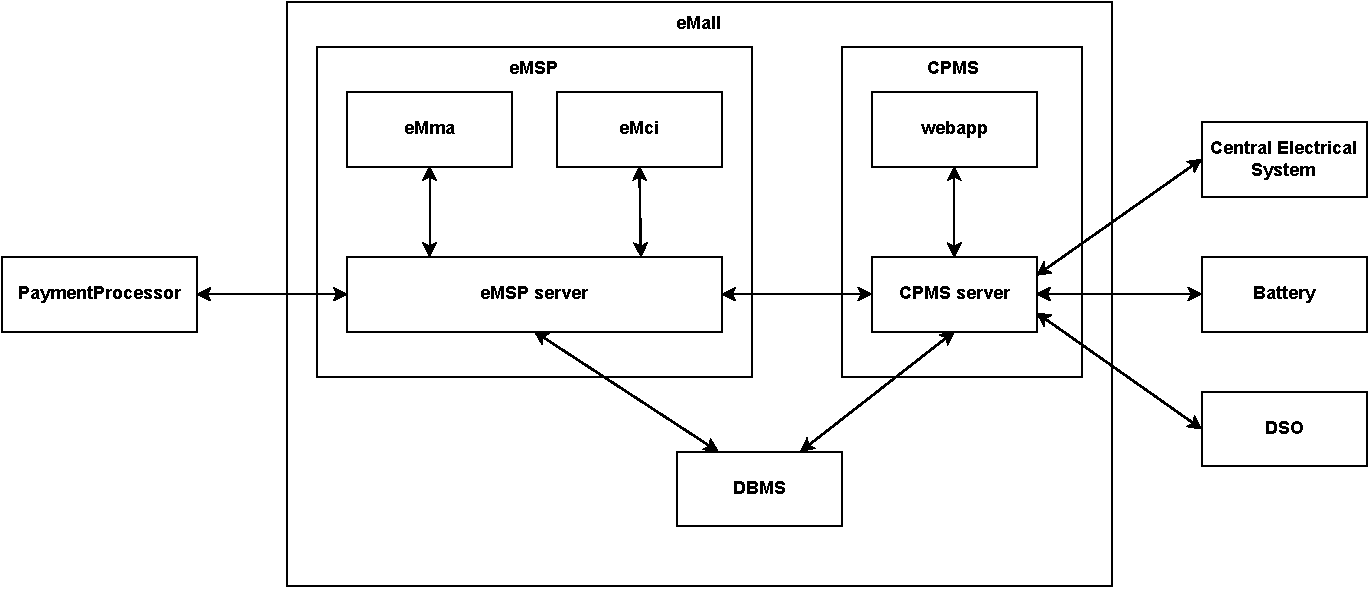
\includegraphics[width=0.8\textwidth]{Images/cp2/overview.pdf}
    \caption{High level description of the components and their interactions}
\end{figure}

\par
%TODO: Bianca please check if you can understand this pargarph
The eMall system, illustrated in the figure, is the objective of this design document. It is clear that the system is divided in two main sub-systems: eMSP and CPMS. This choice is driven by an interoperability requirement of the eMSP and the CPMS with different CPMS and eMSP systems respectively, offered by other companies. Nonetheless, this low-coupling of the CPMS with the eMSP doesn't preclude us from reusing components that have the same functionality in both sub-systems. It is also important to point out that our system, specifically the CPMS sub-system, must be able to interface with the system responsible for managing the technical aspect of the charging point, the system that manages the battery, if present, and the DSO's software system.
\par
As we stated previously, the system has a three-tier architecture. In particular the three tiers are:

\paragraph{Client tier} It's the tier closest to the user and its duty is to manage the user interaction. This means that it must handle the visualization of the content to the user and interpret and translate the user interaction in requests to be forwarded to the application tier. We'd like to remark that this tier doesn't contain any application (or business) logic. We will use a client-side rendering software architecture to design this layer.

\paragraph{Application tier} This is the part where the core and the business logic of the system is implemented, consequently, this second layer realizes the functionalities required to the system, like the booking service or the charging station management service for the CPO. All this functionalities shall be discussed in more detail in the upcoming sections. As we will see in the following section, a micro-services approach has been used to build such layer.

\paragraph{Data tier} The third, and bottom tier, of our system is the data tier, where the persistence concerns of our system are met. The eMall system, both CPMS and eMSP sub-systems, has to handle a large amount of data, which must be carefully stored in order to have a properly working system. The data management is an aspect of software systems that has been thoroughly studied and developed, so the obvious choice for our system is to use an already implemented and tested Database Management System (DBMS).

\section{Component view}
In this section we will discuss and elaborate on the components that compose our system in order to implement the functionalities listed in the RASD document. We will start from a higher level of abstraction to provide a grasp of how the system works, thus even those who are not familiar with the technical aspect of a software system can understand at high level how the system is structured. Afterwards, we will proceed to further analyze the system at finer levels.
\begin{figure}[H]
    \centering
    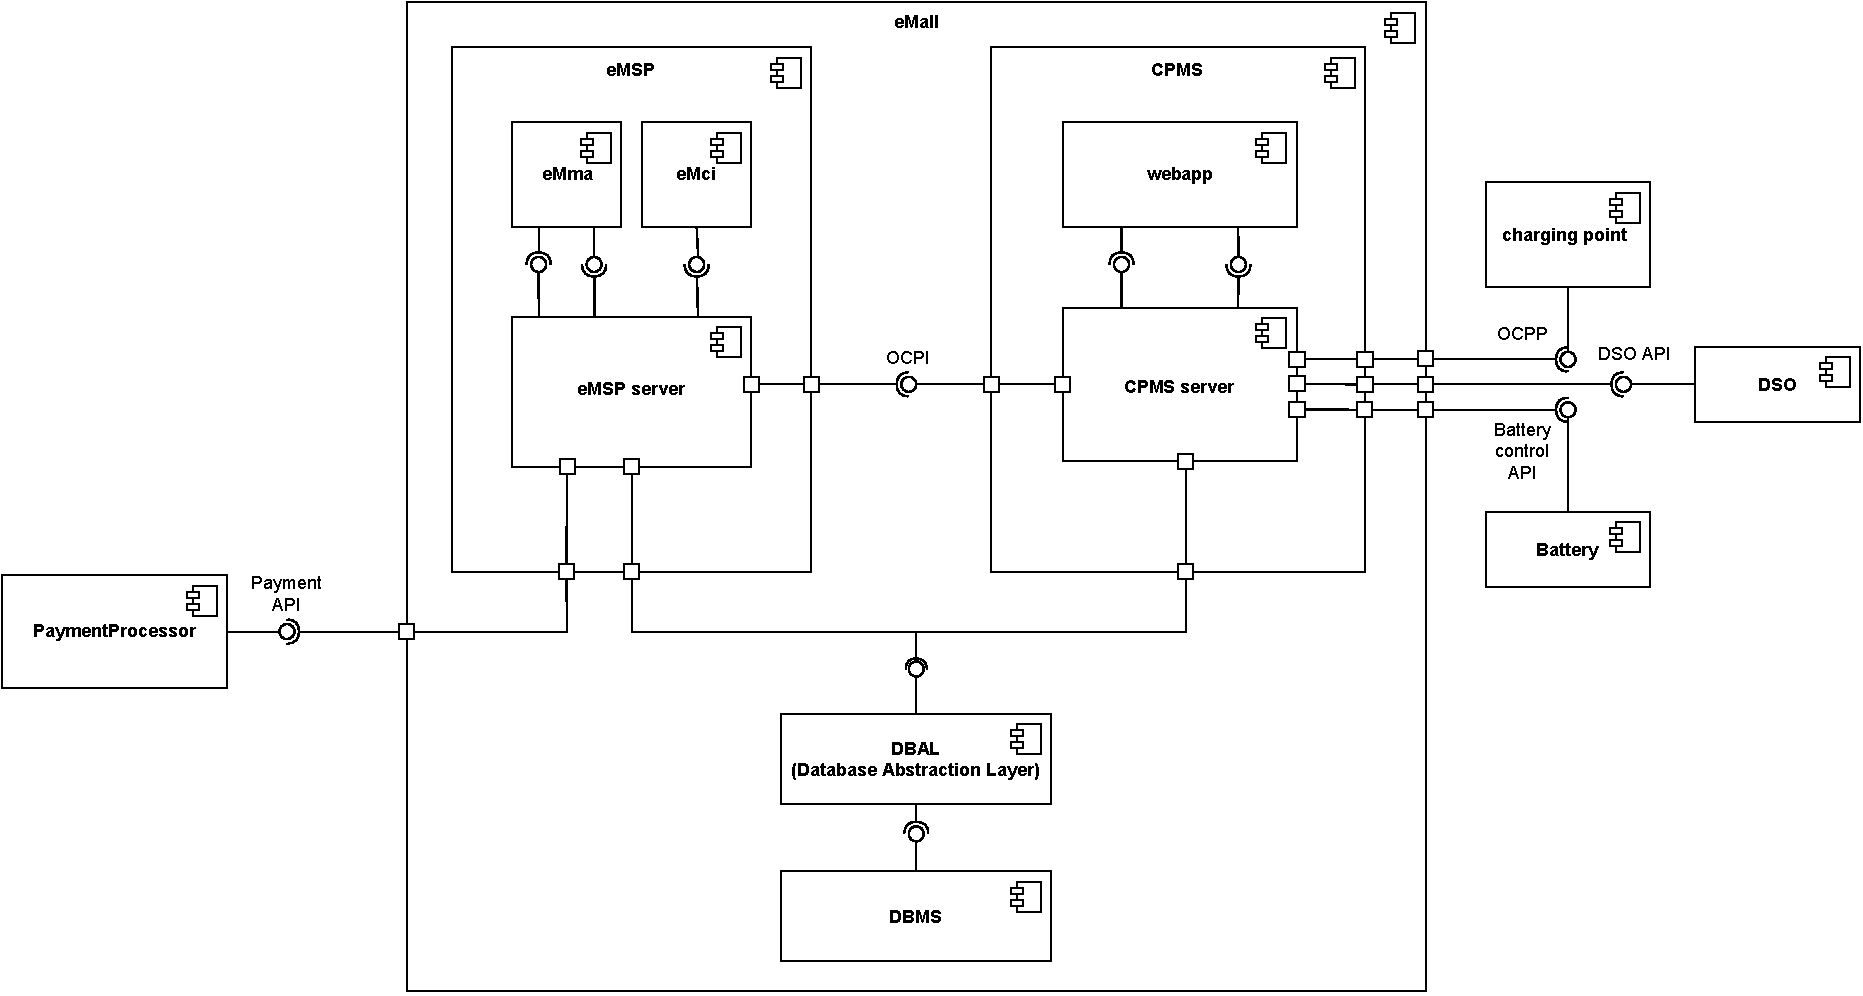
\includegraphics[width=1\textwidth]{Images/cp2/component_overview.pdf}
    \caption{Component view of the system}
\end{figure}

This component diagram provides a higher level view of how the system it is composed. It distinguishes the parts that the development team bust build (the eMall component), and lists the external system with their respective interfaces with which the eMall must interact to provide its functionalities. Furthermore, it's apparent that the system is composed by two main sub-systems, the eMSP and CPMS, that must interact with each other through the OCPI interface, and each of this sub-system is structured in a client-server architecture. The OCPI interface is an open and free interface that standardizes the interface of a CPMS, in other words it standardizes the services a CPSM offers and how to make request for these services to the CPMS. As a consequence of using the OCPI protocol we allow our eMSP to be able to interact with different CPMS\textit{s}, and our CPMS to interact with different eMSP\textit{s}, as per requirement. Finally, there are the DBMS and DBAL components, that compose the third and bottom tier of our architecture. The presence of the DBAL component tells us that a level of indirection from the DBMS has been added, allowing the system to be independent from any particular DBMS.
\par
In the next paragraphs we shall discuss in more detail the composite structure of the main sub-systems of the eMall: the eMSP and CPMS.
\pagebreak

\textbf{eMSP}\\
\begin{figure}[H]
    \centering
    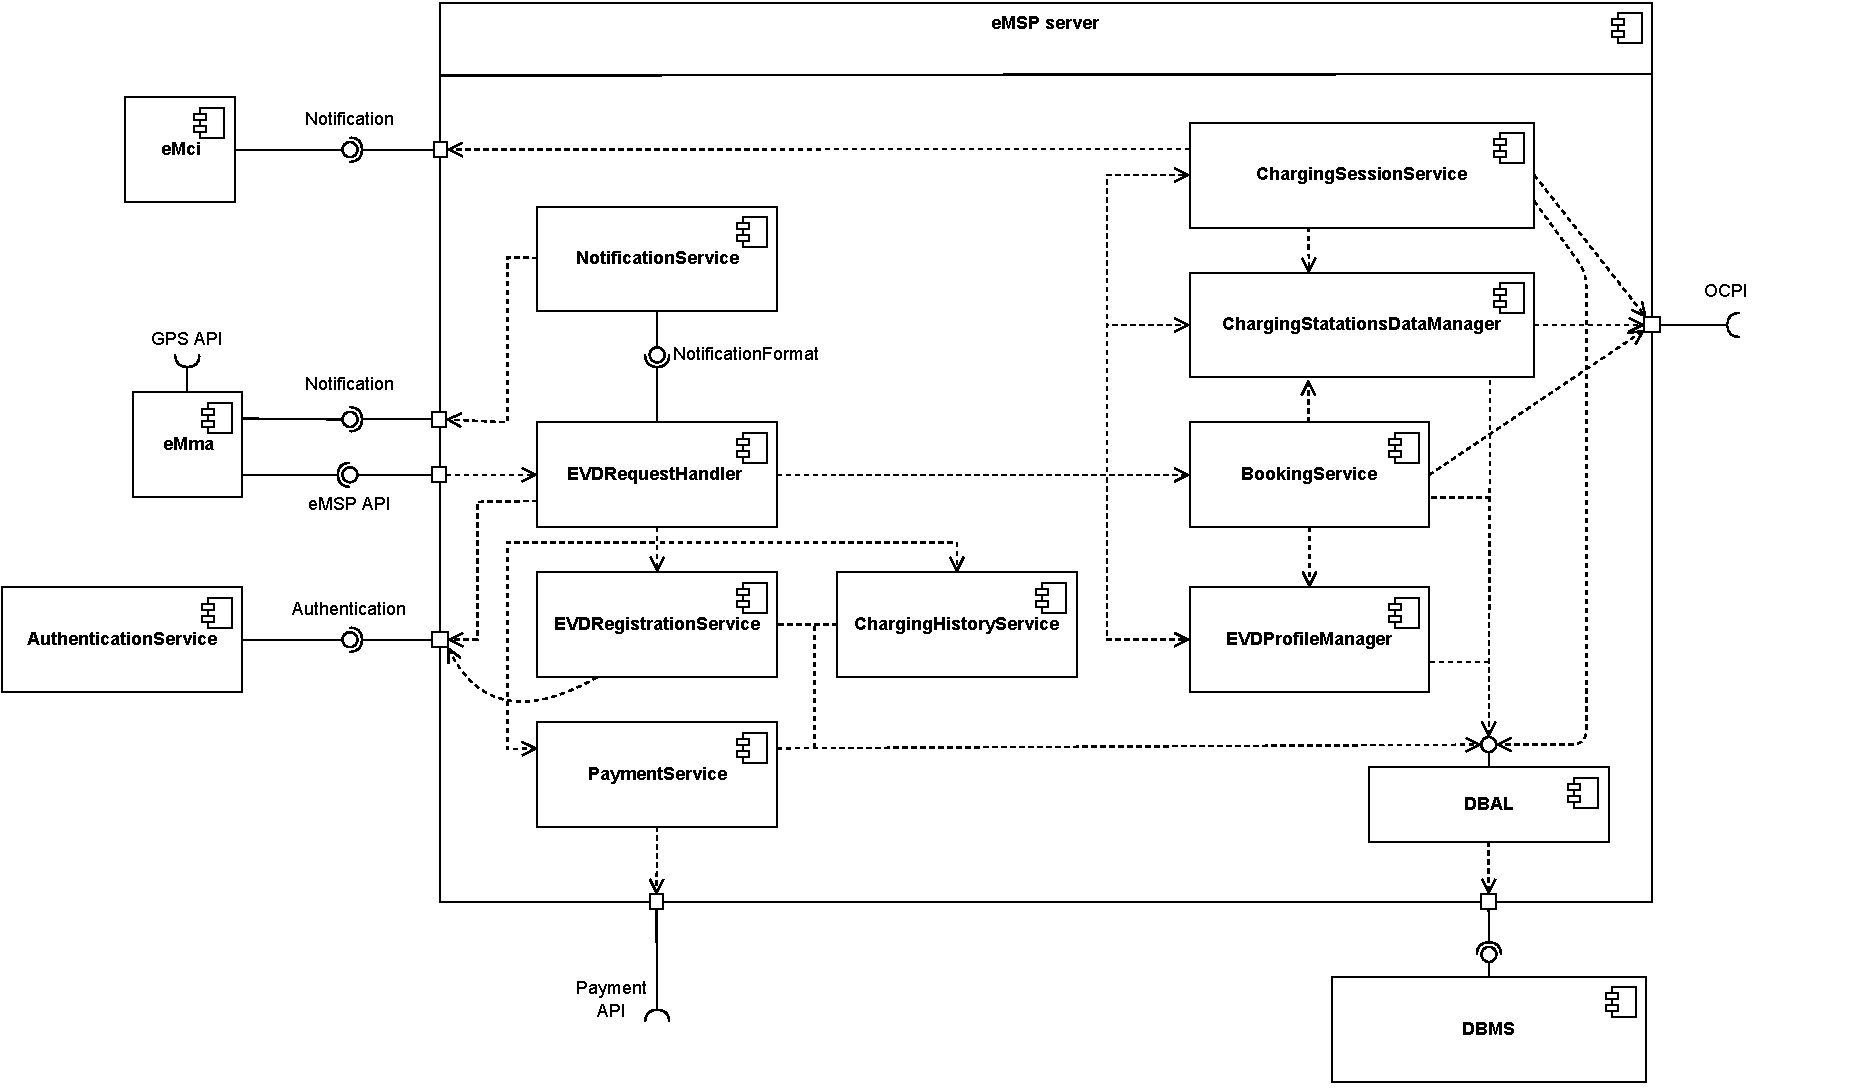
\includegraphics[width=1\textwidth]{Images/cp2/eMSP_server.pdf}
    \caption{eMSP composite structure}
\end{figure}

The eMSP is the system that will interact with the EVD and forward his charging request to the CPMS. As we can see the eMSP isn't only a middleman between the EVD and the CPMS but offers other services like profile management, payment services and charging history services. Below we provide a brief description of each component of the eMSP:
\begin{itemize}
    \item \textbf{eMma}: eMall mobile app. It is the client componet of the eMSP, its task si to act as a view and controller for the EVD interactions. Specifically, it will provide a GUI to the user from which he can make his request to the eMSP. Furthermore it will encode the user input and interaction with the view to the corresponding functions of the eMSP server interface. Finally it has to interact with the GPS module of the OS in which it will run to provide location information to the eMSP
    
    \item \textbf{eMci}: eMall charging interface. This component's role is to provide the graphical interface the EVD will be using at the charging point when he wants to start a charging session and is located on an embedded device on the charging point. It's job is then to identify the charging point in which it resides so the EVD can inform the eMSP of which charging point he wants to use

    \item \textbf{DBMS}: Database Management Service. It is the usual system with the task of managing the insertion, storing, deletion and update of the data generated by the system. This component exceptionally complex and given the widely availability of this kind on systems on the market, using an already build and thoroughly tested one will be mandatory

    \item \textbf{DBAL}: Database Abstraction Layer. It functions as an additional layer of indirection form the DBMS. In this manner the eMSP will be independent of the DBMS used and if this component changes in the future the eMSP won't need to be modified to integrate the interface of the new DBMS

    \item \textbf{AuthenticationService}: Component that has to mange user's authentication to the system and authorization to use the services

    \item \textbf{PaymentService}: This component, through the usage of external Payment API offered by external providers, allows the eMSP to handle the payment requests from the users

    \item \textbf{ChargingHistoryService}: The component which has to process the data saved in the DB to present the user with a functional information regarding his charging history

    \item \textbf{EVDRegistrationService}: Component which has to handle the user registration process. Obviously it shall use the the DBAL to store the user information once the process has finished. Additionally it also has to use the component AuthorizationService in order to login the user once the registration process has successfully ended

    \item \textbf{EVDProfileManager}: Component responsible for managing and processing the data concerning the EVD personal information and the EVD's data about his EVs

    \item \textbf{ChargingStationsDataManager}: This is one of the main components of the system. It has to interact with the CPMS to gather data useful for the EVD and more specifically that will be used and processed by the other components. Moreover it acts as an interface for other components that need information about the stations, so don't need to depend on the data structure used to store the stations

    \item \textbf{ChargingSessionService}: Component responsible for unlocking the charging point, starting the charging session and terminating it. Obviously to offer this services it must interact with the CPMS trough the OCPI interface. Additionally it uses the DBAL interface in order to save the data about the charging session, which will be used by the ChargingHistoryService component, and can perform checks when the user is trying to unlock the wrong charging point by cross-checking the data stored in the DB about the charging points and the code it receives by the eMci component

    \item \textbf{BookingService}: Component that provides the booking functionality. It must use the EVDProfileManger and the ChargingStationsDataManager components to get the specific information about the user and the station respectively in order to make the appropriate request through the OCPI interface. Moreover it stores this information in the DB so that when can be used to cancel a booking
    %TODO: if the OCPI doesn't allow to cancel a booking and allows only booking within 15 min what we do, we have to change requirements and functionalities. Or we can accept the booking, wai and try booking through the CPMS when the time comes (needs to send notification if it doesn't succeed).
    
    \item \textbf{NotificationService}: Component that provides the eMSP server with the capability of sending notification to the EVD through the eMma component, consequently this component must use the communication interface offered by eMma

    \item \textbf{EVDRequestHandler}: All the users' requests pass trough this component. This centralized approach is need so the system can check if the requests have the right permissions (i.e. request for services allowd only for registered user). This explains the dependency with the AuthenticationService component. Obvioulsy it also need to use all the other components to grant the user the services offered by the system

\end{itemize}
\pagebreak

\textbf{CPMS}\\
\begin{figure}[H]
    \centering
    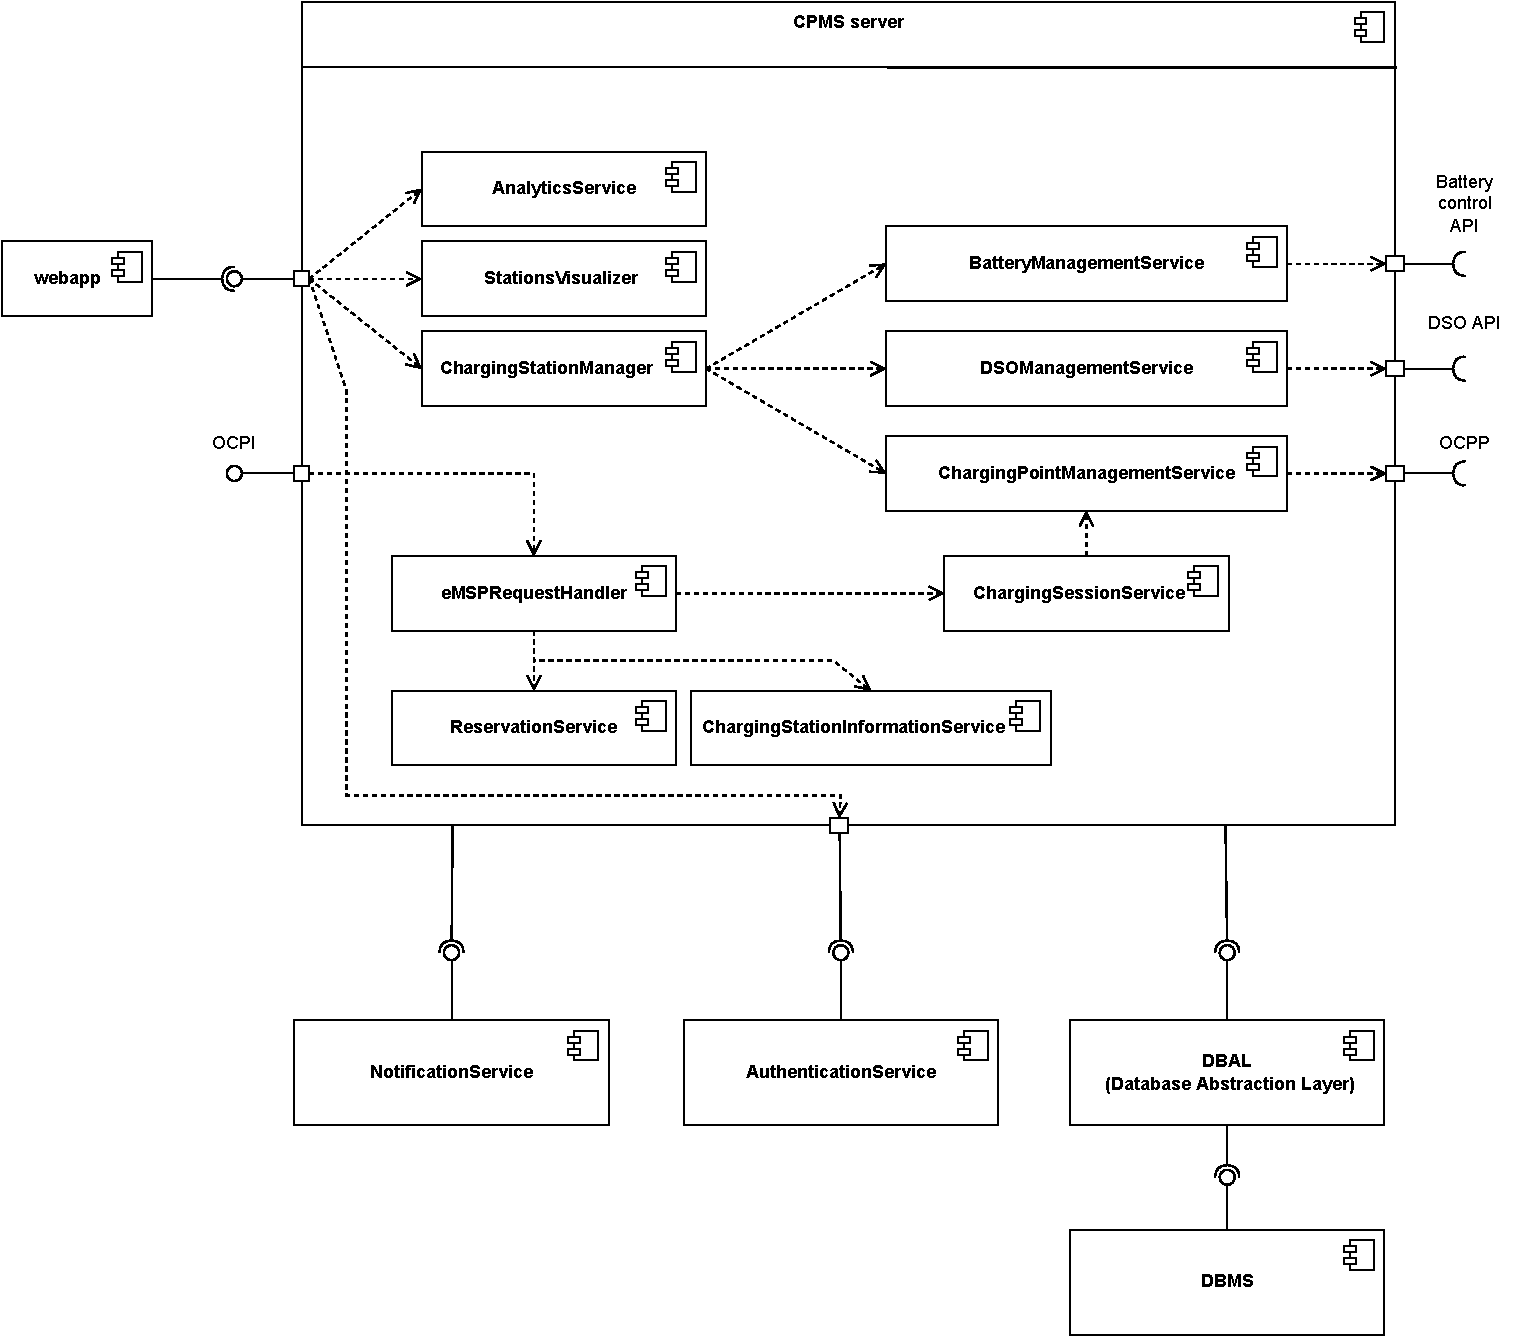
\includegraphics[width=1\textwidth]{Images/cp2/CPMS_server.pdf}
    \caption{CPMS composite structure}
\end{figure}

The CPMS is the subsystem responsible for manging the charging station, offering charging services to EVDs and securing the electricity supply from the DSOs. To offer all this functionalities this sub-system of the eMall must collaborate with other systems external to our own, which can be viewd in the general overview. Specifically, the CPMS needs to interfaces to the system responsible of managing the battery by the \verb|Battery control API| interface, with the DSO IT system through it's API and with the the system managing the charging points devices through the protocol OCPP, which is an open standard. Like we have done for the eMSP, we will proceed describing each component of the CPMS sub-system (components AuthenticationService, DBAL, DMBS and NotificationService have the same functionality as in the eMSP system and shall not be repeated here):

\begin{itemize}
    \item \textbf{ChargingPointManagmentService}: Component responsible for interacting with the central management system of charging station. This component will query this central system through the OCPP protocol, asking for the status of the charging points, and invoking request like starting (likewise terminating) the flow of electricity of a particular charging point to start a charging session

    \item \textbf{DSOManagementService}: Component responsible for collecting the data from the various DSO and concluding sales contracts with them if the API allows it

    \item \textbf{BatteryManagementService}: Component responsible for managing the battery of the charging station if one is present. This component must interface with the software system managing the technical aspects of the battery trough its control API (here called Battery control API) and must use the methods provided by the ChargingPointManagemntService component to allow the central system to switch to the battery for charging or charging the battery when requested

    \item \textbf{StationsVisualizer}: Component that allows the CPO to visualize and select one of the charging stations managed by him

    \item \textbf{AnalyticsService}: Component that provides the CPO with the tools to do some statistical analysis on the data collected by each charging station

    \item \textbf{ChargingStationManager}: Main component responsible for the interaction with the CPO. It implements all the functionalities related to the business aspect of the charging station (setting electricity price, promotions, etc.) and uses the component described before for managing the technical aspects of the charging station. This component also uses the NotificaionService component to notify the CPO about any necessary information

    \item \textbf{CPORequestHandler}: It is the component where all the CPO request must first pass trough in order to perform security checks and allow only authorized user to access the services of the CPMS. To offer this functionality the component makes use of the AuthenticationService component to login the user and to check if the request coming from the webapp have the necessary authorization. If a request passes the controls it's forwarded to the respective component

    \item \textbf{ChargingSessionService}: Component responsible for handling the starting, monitoring and terminating of a charging process

    \item \textbf{ChargingStationInformationService}: Component in charge of processing the data of the charging station, stored in the DB, in a suitable format for the eMSP and compatible with the OCPI interface

    \item \textbf{ReservationService}: Component responsible of managing the reservation of the charging points 

\end{itemize}

\section{Deployment view}
\begin{figure}[H]
    \centering
    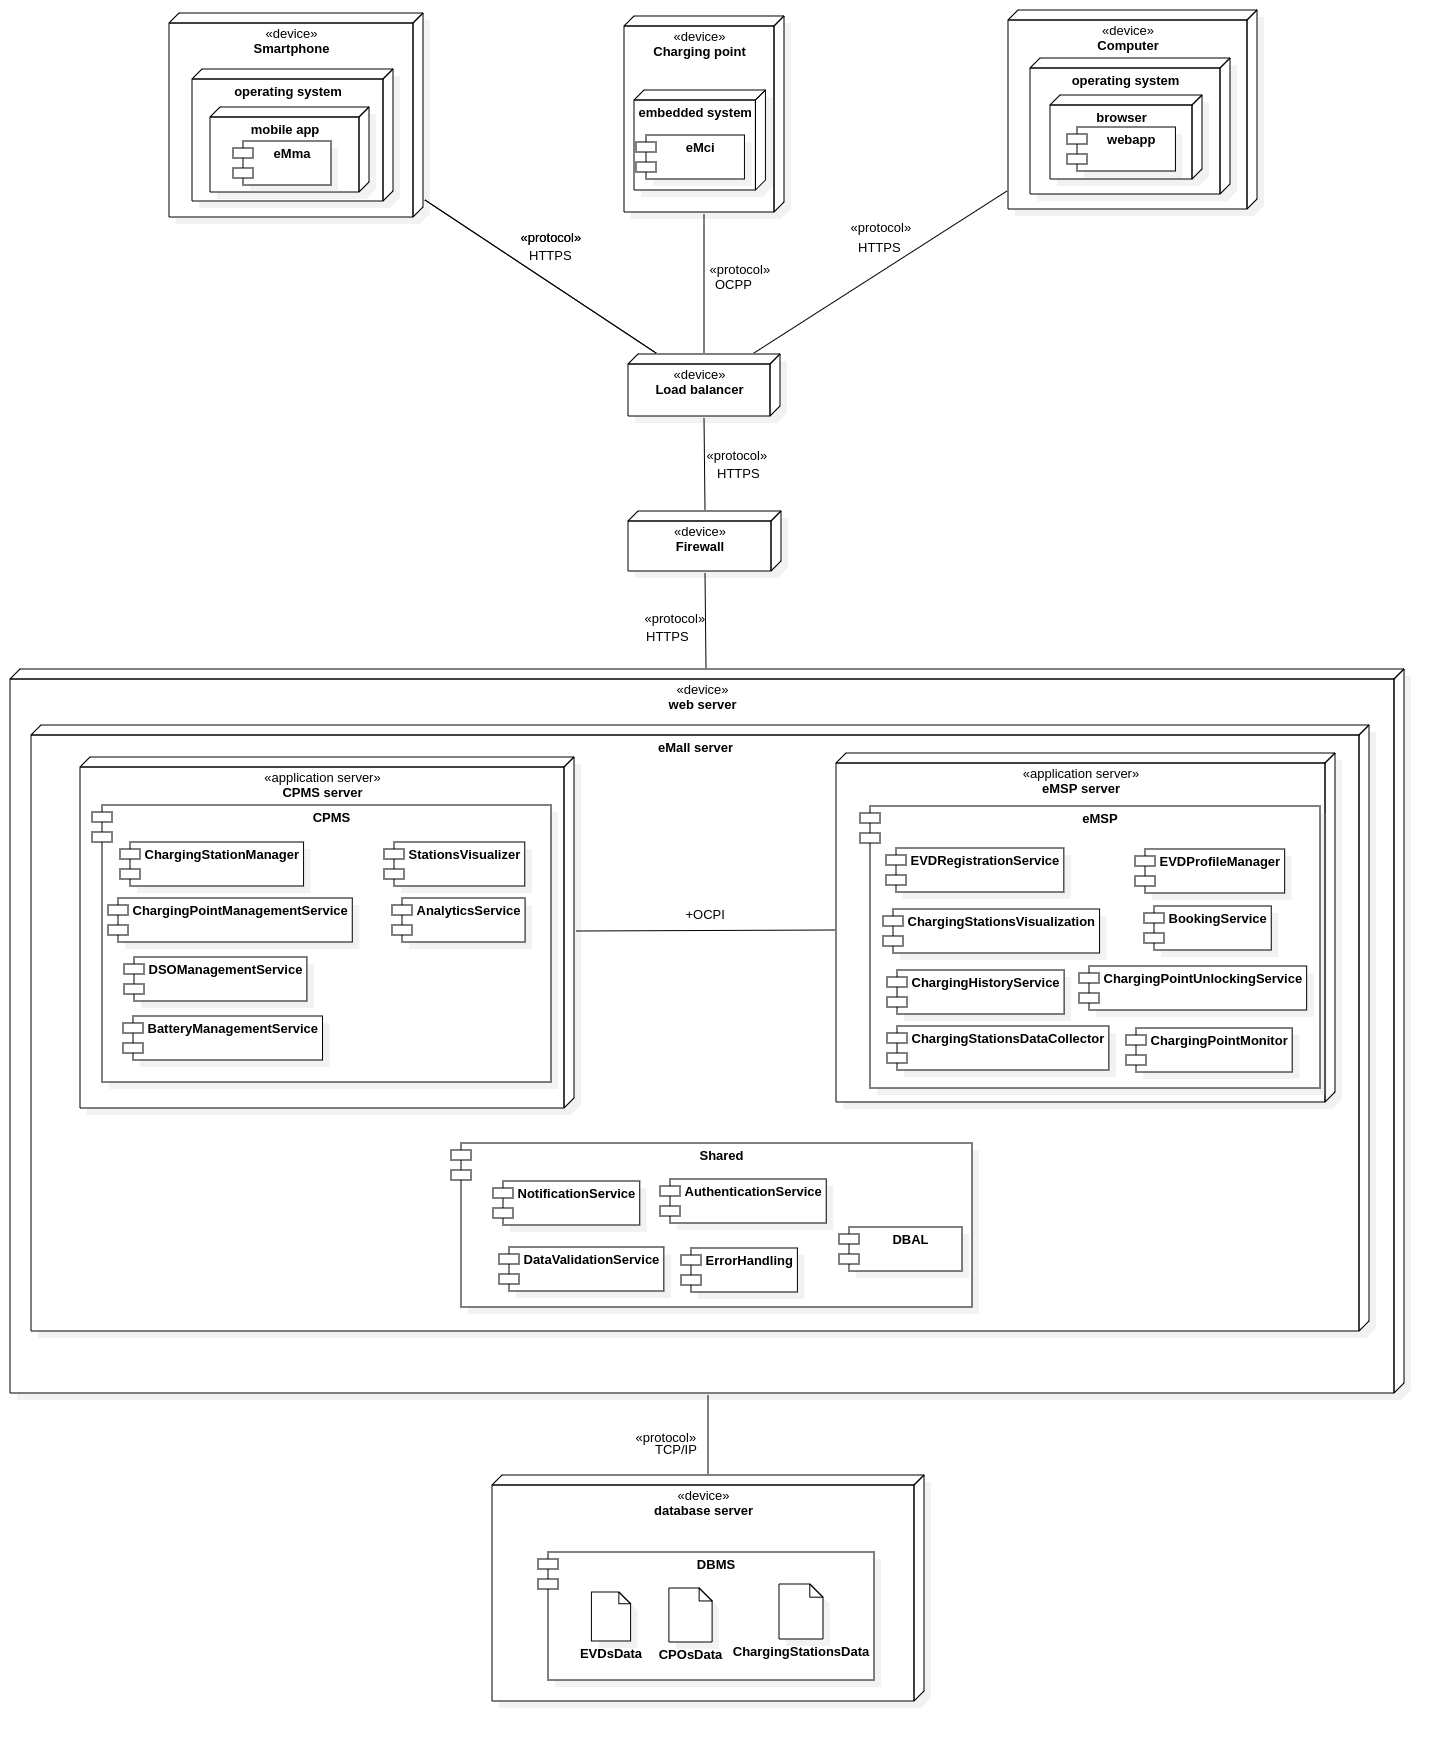
\includegraphics[width=1\textwidth, height=0.9\textheight]{Images/cp2/DeploymentDiagram.png}
    \caption{Deployment view of the system}
\end{figure}
At the client level we can see three different devices interacting with the system:
\begin{itemize}
    \item \textbf{Smartphone} - The smartphone runs the mobile application of the eMall, the eMma, and has internet access in order to send the HTTPS requests to the system. This is the kind of device used by the EVDs that use the eMall
    \item \textbf{Computer} - The computer runs the web application of the eMall, and also has internet access to manage the service through HTTPS requests to the system. This is the kind of device used by the CPOs of the companies that use the eMall to manage their charging stations
    \item \textbf{Charging Point} - The charging point is the specific device used by the EVDs to charge the EVs and it has an embedded system, which through the OCPP protocol communicates with the CPMS part of the eMall system, in order to correctly provide the charging service
\end{itemize}

Between the client level and the application level, we have some architectural elements that allow to achieve some non-functional requirements, such as better performance, scalability, availability and security:
\begin{itemize}
    \item \textbf{Load balancer} - The load balancer is a network device that distributes incoming requests across a group of servers to help improve the performance and availability of the application. A load balancer can help to improve the performance of the application by distributing incoming requests across multiple servers, rather than routing all requests to a single server. This can help to prevent any single server from becoming overloaded, which can improve the overall responsiveness and performance of the application. A load balancer can make it easier to scale the application horizontally by allowing to add or remove servers as needed and this can be useful if we need to add more capacity to handle a growing number of users. A load balancer can, also, help to improve the availability of the application by routing traffic to a healthy server in the event that one of the servers becomes unavailable. We can see that the load balancer is useful to improve different non-functional requirements of the eMall, that can be implemented using different servers to have better characteristics 
    \item \textbf{Firewall} - The firewall allows to protect the network from external threats and unauthorized access, blocking incoming traffic that does not meet the security rules. The firewall is necessary in order to comply with certain regulations and industry standards, because we are handling sensitive data (financial information, personal data), so is necessary to protect the data. The firewall can also help to improve the performance of the application by blocking traffic that is not necessary or relevant to the application, improving the overall responsiveness of the eMall
\end{itemize}

The eMall web application and mobile application provide both static and dynamically generated content, so the system runs web servers for the static content and application servers to generate content dynamically. The load balancer sends to the web server the HTTPS requests that need only static content, and on the other side sends to the correct application server the requests to generate the dynamic content and accomplish more complex functionalities due to the interaction of the eMall components. 
At the application level the deployment diagram shows in a simplistic way the following elements:
\begin{itemize}
    \item \textbf{Web server} - For the web server we have a computer that stores software and website raw data, such as HTML files, images, text documents, and JavaScript files. The hardware of the web server is connected to the web and supports the data exchange with different devices connected to the Internet
    \item \textbf{Application server} - In the deployment diagram on the same hardware we also have the application servers, one for the CPMS and one for the eMSP, with also the shared services. The application servers contain different micro-services, that interact among them and with external APIs, as shown in the previous component diagram. The micro-services could also be implemented on more servers, splitting the eMSP and CPMS application servers in more servers, or creating a redundancy of the available services on different machines to improve performance and availability, exploiting even better the load balancer
    \item \textbf{Shared components} - The shared components shown in the diagram are components that belong to the two application servers, but also to the web server. The web server of the eMall handles part of these functionalities, sending the rest to the application servers  
\end{itemize}

Finally at the lowest level we have the persistent part of the system, which interacts with the eMall trough TCP/IP and is hidden to the higher levels due to the use of the DBAL. The Database level is composed by:
\begin{itemize}
    \item \textbf{Database server} - It hosts the database of the system and manages the different data through a DBMS 
    \item \textbf{Database artifacts} - The different database artifacts shown in the diagram represent physical implementations of the DB, an implementation for the data regarding the EVDs, one for the companies and CPOs data and finally an implementation for the data regarding the charging stations and any other related data
\end{itemize}
For a more secure system we consider not only a DB, but also some replicas, distributed on different machines to guarantee more availability, fault tolerance and disaster recovery. 

\section{Runtime view}

\section{Component interfaces}

\section{Selected architectural styles and patterns}

\section{Other design decisions}


\chapter{User Interface Design}
\label{ch:chapter_three}%
\section{EVD user interface}
\subsection{Log in}
\begin{figure}[H]
    \centering
    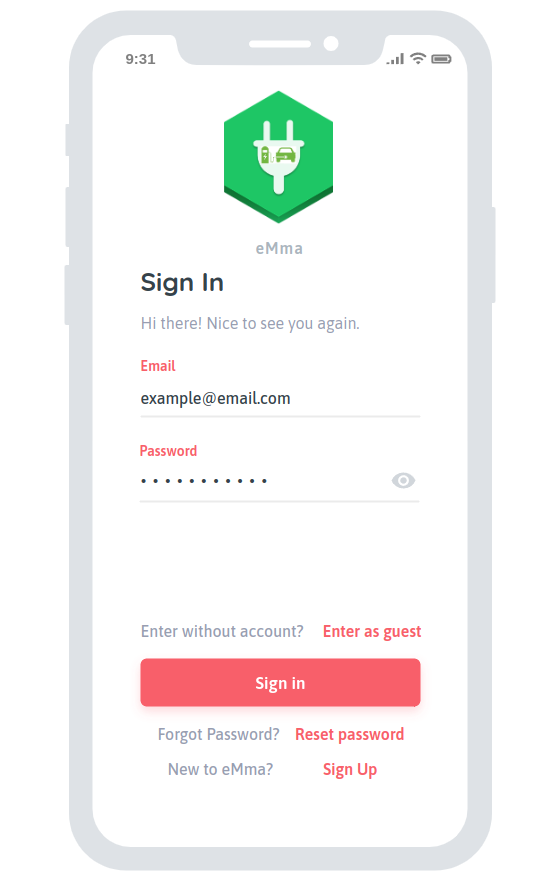
\includegraphics[width=0.4\textwidth]{Images/cp3/logIn.png}
    \caption{UI for the log in}
\end{figure}
We can see from the UI for the log in that the operation is very simple. To sign up is enough to enter the email and the password used during the registration. The EVD can enter into eMma as a guest, if he doesn't want to sign up, but in that case it will perceive only some limited functionalities of the application. It can also be useful to set a mechanism to manage the case in which the user forgets his password.

\subsection{Register}
\begin{figure}[H]
    \centering
    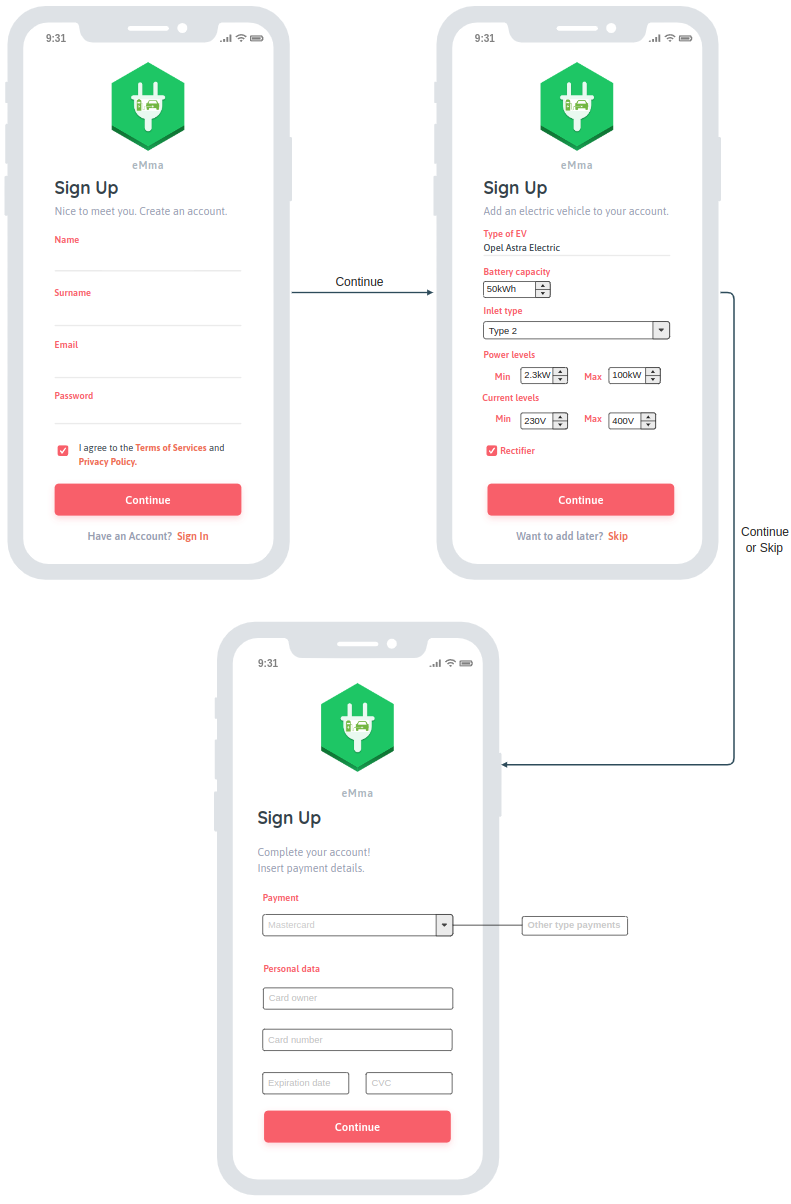
\includegraphics[width=0.85\textwidth]{Images/cp3/registerMockup.png}
    \caption{UI for registration}
\end{figure}
The UI for the registration was thought in order to be as user-friendly as possible. First, to sign up is necessary to insert some personal data, such as the name, the surname, and the email and password that will be used for the log in, as previously explained. It is also necessary to accept the 'Term of Service' in order to continue with the registration. The second step asks the user to add some data about his EV and we can see that the insertion is guided by the interface in order to avoid as much as possible data errors. The EVD has to add the type of the EV, the inlet type, the power levels and the current levels, and has to check or not the final box to inform if the car has or not the rectifier. Finally, to complete the sign up process the user is requested to insert the payment details. After registration, from the personal profile the EVD will be able to add new data to his profile, such as new payment methods and new EVs, and he will be able to modify these ones.

\subsection{Charge now}
\begin{figure}[H]
    \centering
    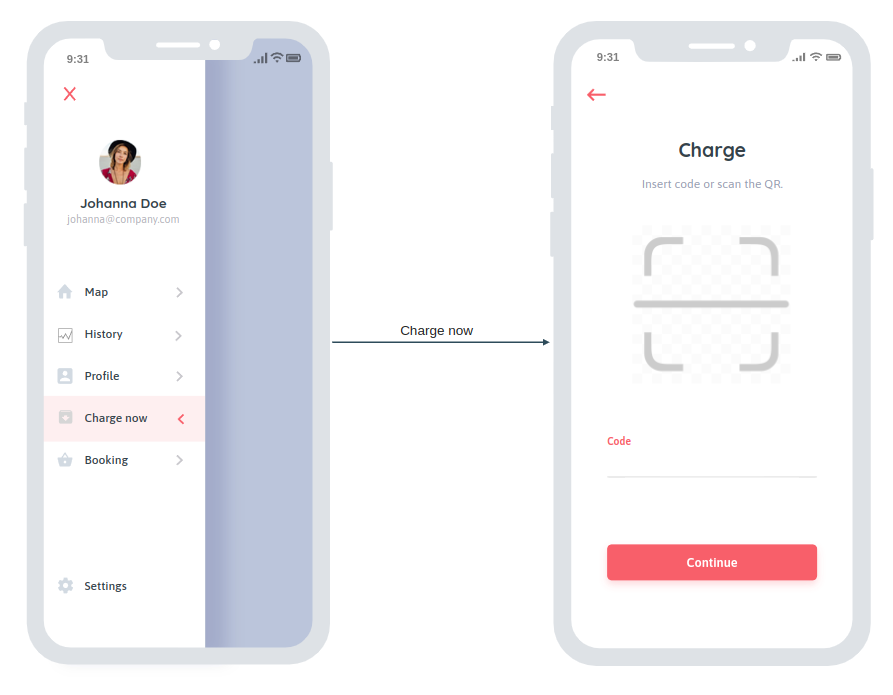
\includegraphics[width=0.85\textwidth]{Images/cp3/chargeNow.png}
    \caption{UI for starting the charging session}
\end{figure}
To start the charging process the EVD has to insert the code or scan the QR present on the charging point. This can be started from the menu or from the 'Charge now' button present in the charging station page, as we will see in the following mock-ups. 

\subsection{Visualize stations}
\begin{figure}[H]
    \centering
    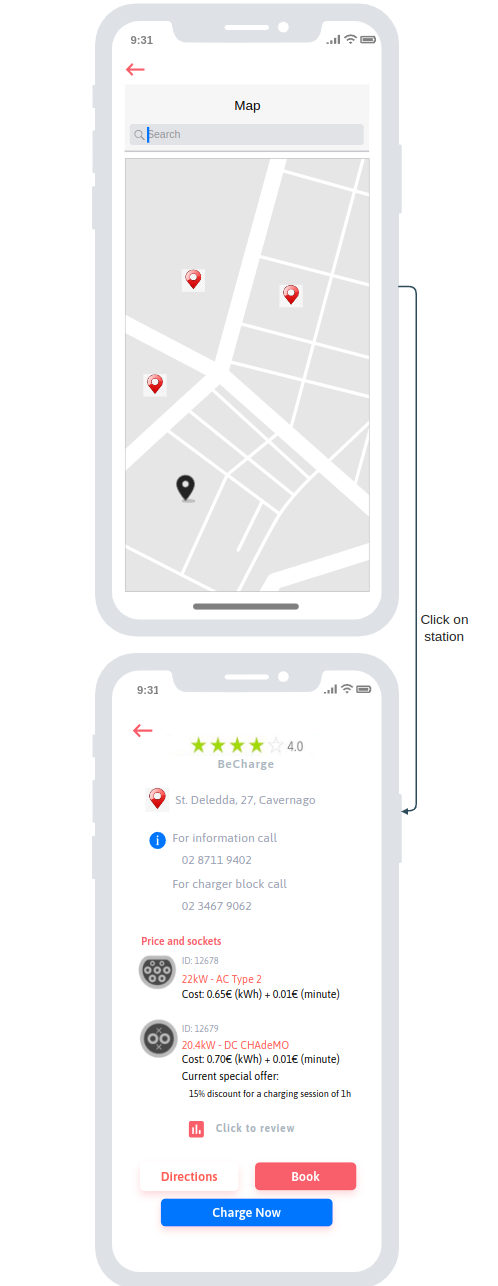
\includegraphics[width=0.4\textwidth]{Images/cp3/visualizeStations.png}
    \caption{UI to visualize stations on the map and their information}
\end{figure}
The main page of the eMma shows to the user the map and permits to visualize the charging stations nearby or to insert a position in which to search for new stations. Clicking on one of the stations, the application shows the charging station page with the most important information: the rating, the name of the station, the address and the contacts, the available sockets and the respective prices and special offers. Finally, it is possible to leave a review or to see the ones left by other users. From this page is possible to get the directions to reach the station and it is also possible to start the main operations of the system: the charging session and the booking of a charging point.

\subsection{Booking charging point}
\begin{figure}[H]
    \centering
    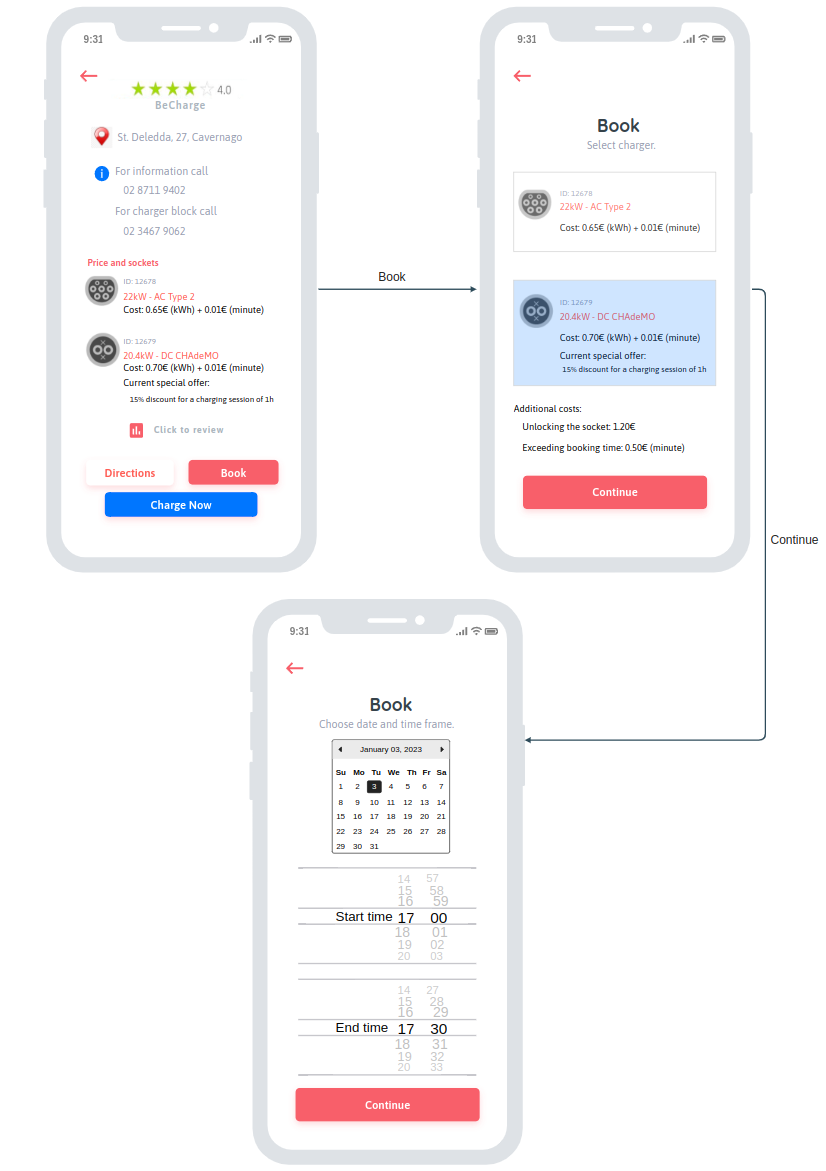
\includegraphics[width=0.75\textwidth]{Images/cp3/bookingCP.png}
    \caption{UI to book the charging point in a certain time frame}
\end{figure}
During the booking operation the EVD has to select the charging point he wants to book from the selected station and also to insert the date and the time frame of the booking. 

\subsection{Terminate charging}
\begin{figure}[H]
    \centering
    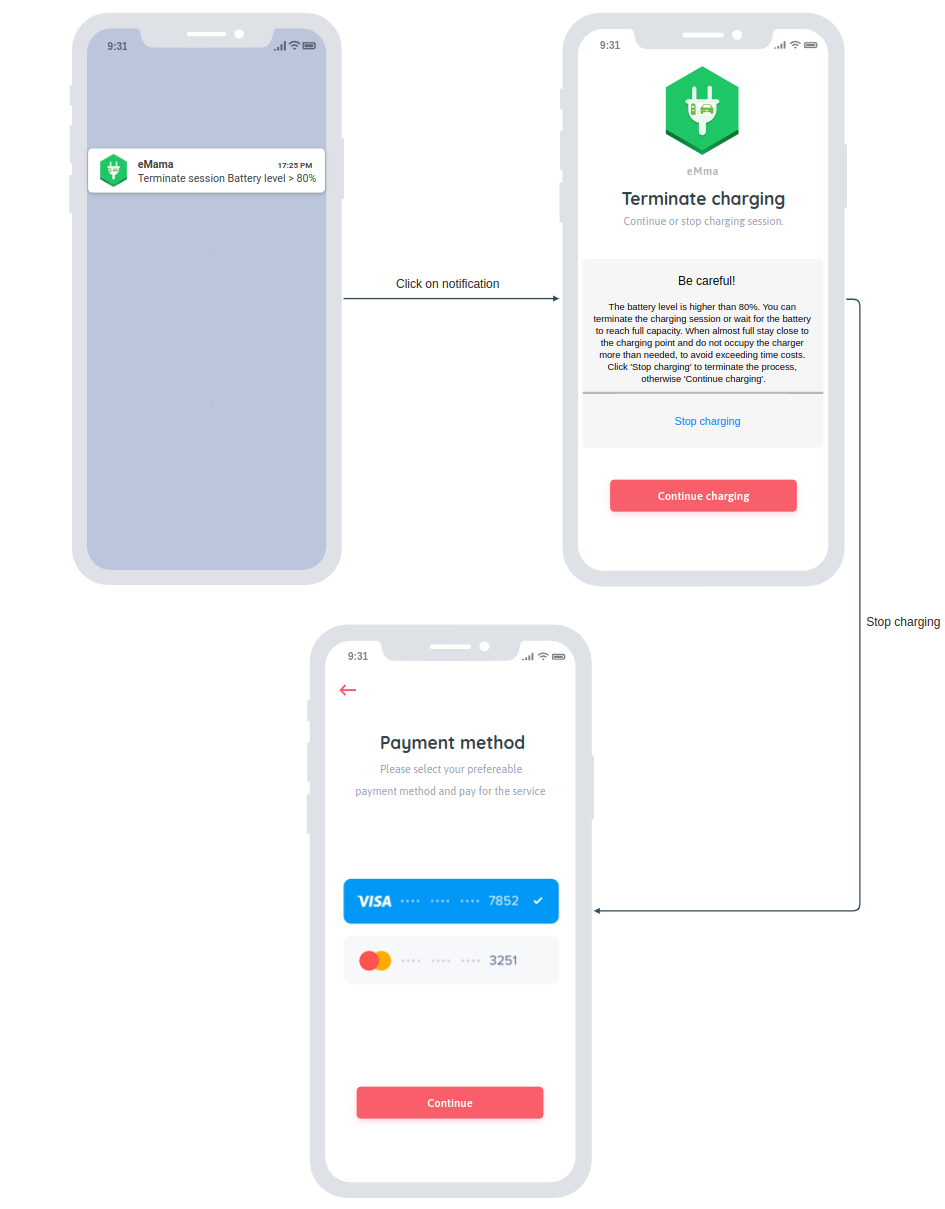
\includegraphics[width=0.9\textwidth]{Images/cp3/terminateCharging.png}
    \caption{UI to terminate the charging session}
\end{figure}
We can see from this UI, that the eMma sends a notification to the user smartphone when the battery level reaches 80\%. The user can decide if he wants to stop the charging session or proceed with the charging until full battery. When the EVD decides to terminate the charging the eMma asks to select the payment method in order to pay for the service.

\clearpage
\section{CPO user interface}
\subsection{Visualize stations and add a general promotion}
\begin{figure}[H]
    \centering
    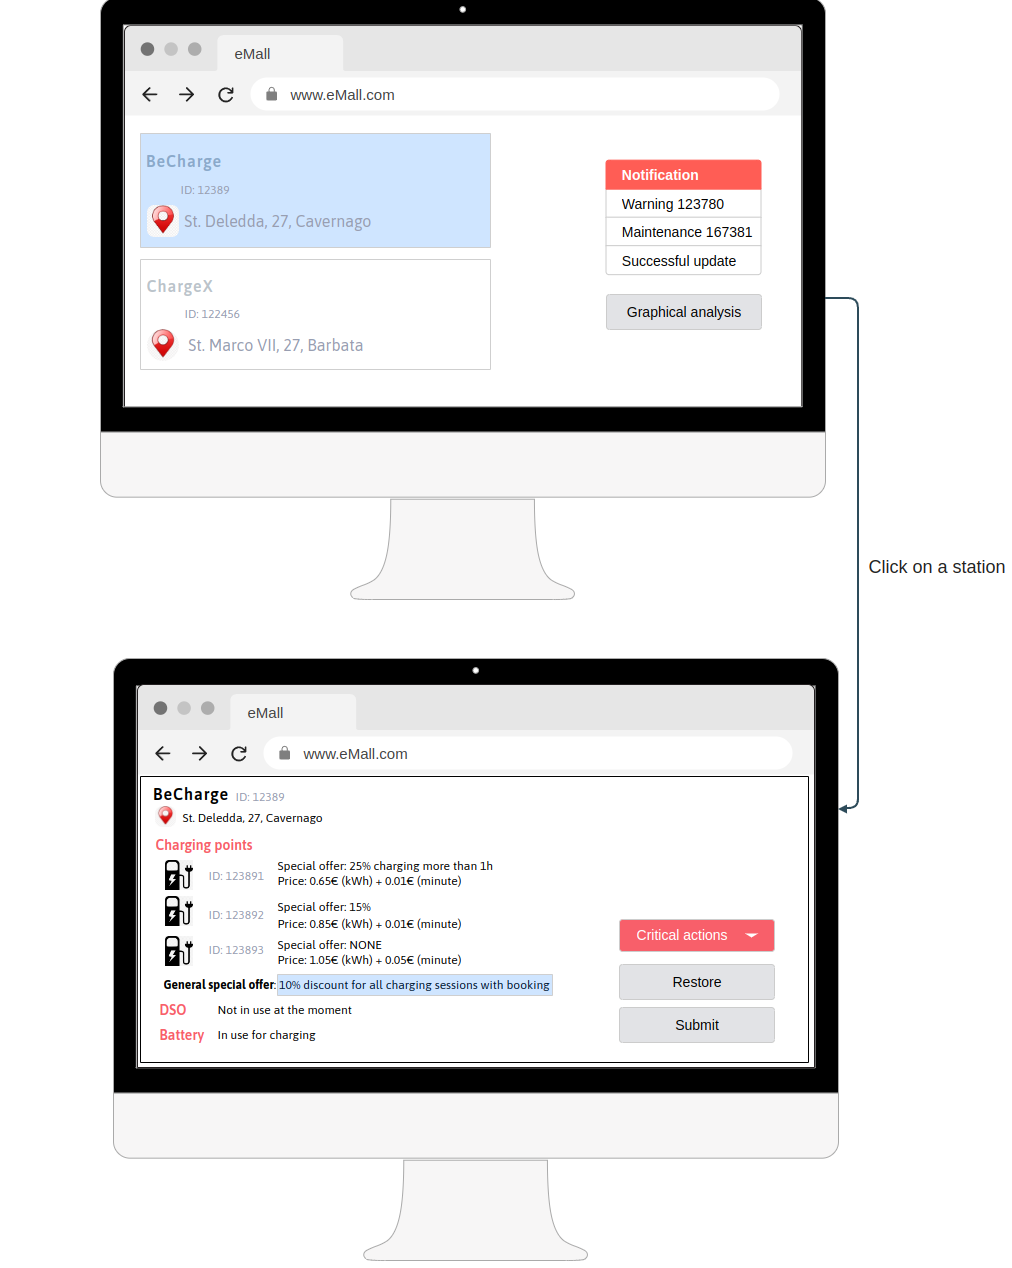
\includegraphics[width=0.75\textwidth]{Images/cp3/setPromotion.png}
    \caption{UI for visualizing the stations and adding a new promotion}
\end{figure}
In this minimal example of UI for the CPO we can see how the homepage allows to visualize the stations that the company is managing, and also presents the notifications sent by the system with a different specification and code, showing a precise communication type and the charging station it is related to. From the homepage the CPO can start the graphical analysis of the stations, can solve a notification and he can also select one of the stations to make some changes. In this case the CPO selects a station and the web app processes the request returning the page with the form related to the specific station. In the form a lot of data can be updated and added to manage the station and in this case the CPO adds a general special offer for the entire station and this will update the prices following the conditions of the promotion. Then the CPO submits the form and waits for a message that informs him of the success of the operation. From the station form is also possible to perform some critical actions, such as deleting the station, deleting a charging point or adding a new charging point.

\subsection{Update price}
\begin{figure}[H]
    \centering
    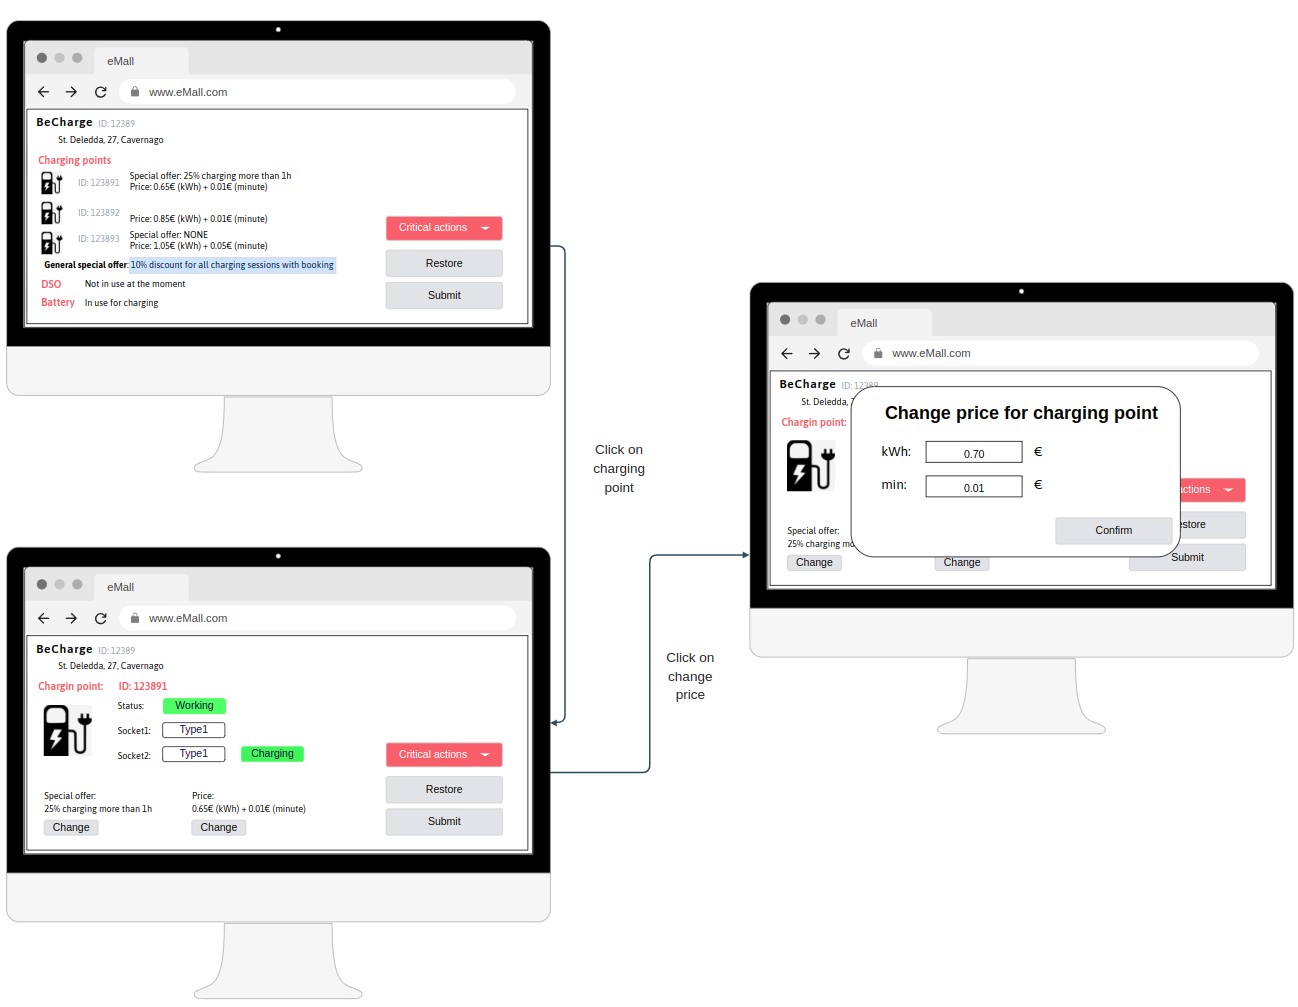
\includegraphics[width=1\textwidth]{Images/cp3/updatePrice.png}
    \caption{UI for updating the price of a charging point}
\end{figure}
From the homepage of a charging station the CPO can select a charging point to have a better view of its specifics. After clicking on charging point, the webapp loads a new page where the details of the device are shown. Specifically, the page shows the status of the charging point (working, off, not activated, etc.), its sockets with the respective type and if they are currently used for charging. In the section below the CPO can see the price set for the charging point and any special offer set on it. From this section the CPO, clicks the button to change the price and a popup comes up where he can insert the new price for the charging point. After entering the new price the CPO must confirm his entries by clicking on the Confirm button. Afterwards, the pop-up closes and the page of the charging point is reloaded with the new information. From this page the user can choose whether to confirm the changes, by clicking on the submit button, or undo the changes by clicking the restore button.

\subsection{Store energy in battery}
\begin{figure}[H]
    \centering
    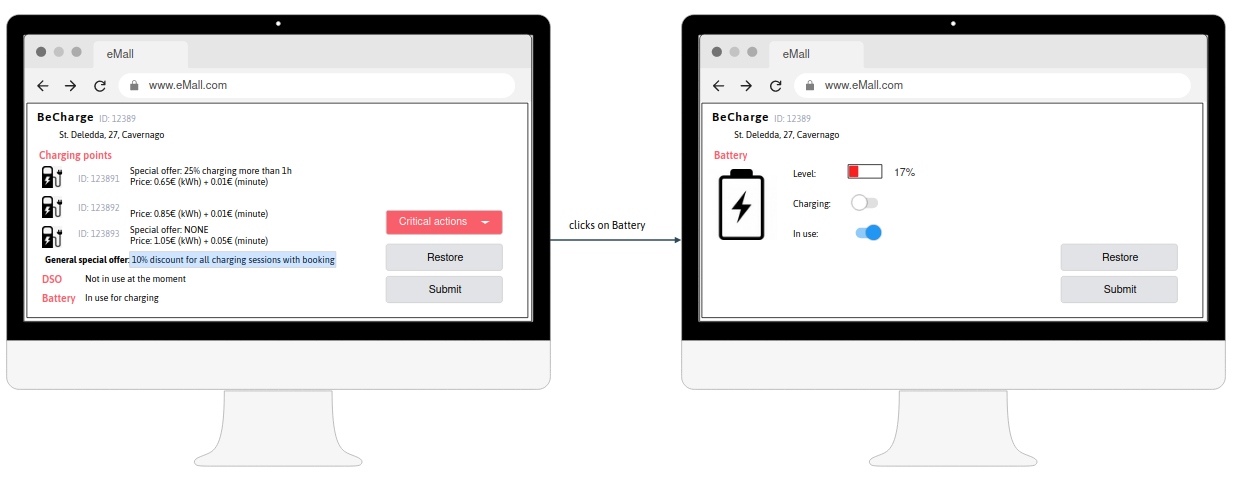
\includegraphics[width=1\textwidth]{Images/cp3/storeEnergyInBattery.png}
    \caption{UI for storing energy in battery}
\end{figure}
Same as before, the interaction with the CPO starts from the homepage of a charging station. From here the CPO can select the Battery text (if present), which will load the page for managing the battery of the charging station. This page shows the percentage of charge left in the battery, if the battery is charging and if the battery is currently in use. By clicking on the toggle \textit{Charging} the CPO can connect the battery to the grid and start charging it.

\subsection{Update DSO}
\begin{figure}[H]
    \centering
    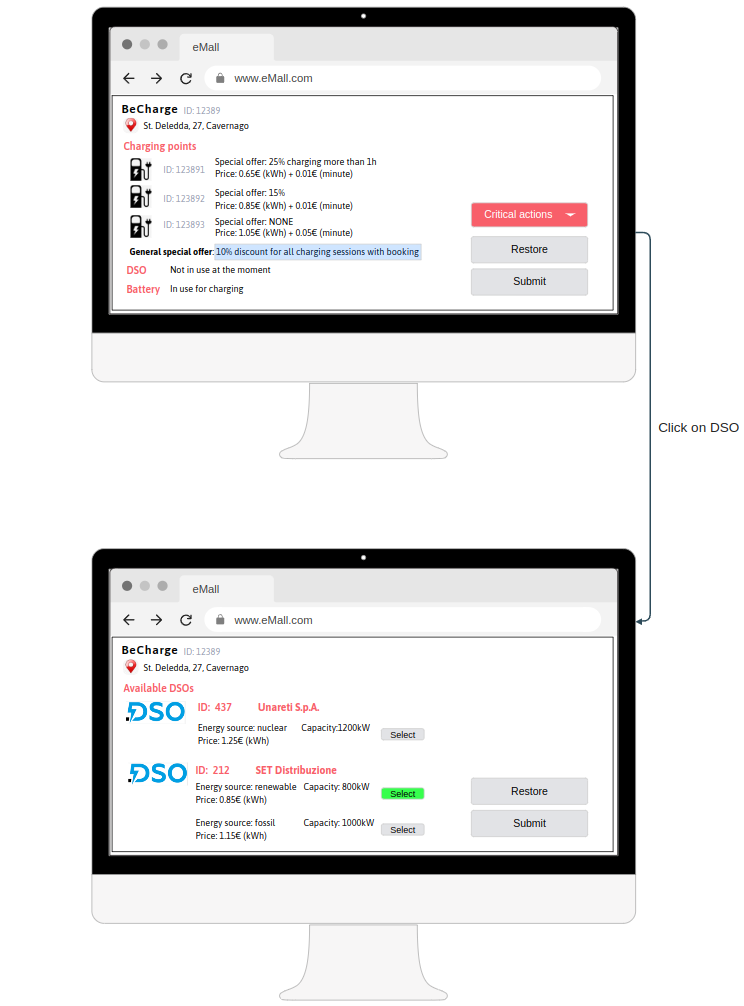
\includegraphics[width=0.73\textwidth]{Images/cp3/updateDSO.png}
    \caption{UI for updating the DSO of a charging station}
\end{figure}
Once on the charging station form is possible to select the DSO and update it or add it for the first time. Clicking on the DSO a new form is loaded in which the CPO can choose one from the available DSOs. For each one of them he can see the energy sources with the respective price and capacity. Is enough to select one DSO with the relative energy source and click the 'Submit' button. Then, a request will be sent to the CPMS part of the system, which will communicate through the DSO API with the external chosen DSO to update the contract, and will also save the new information on the DB. 

\subsection{Analyse stations}
\begin{figure}[H]
    \centering
    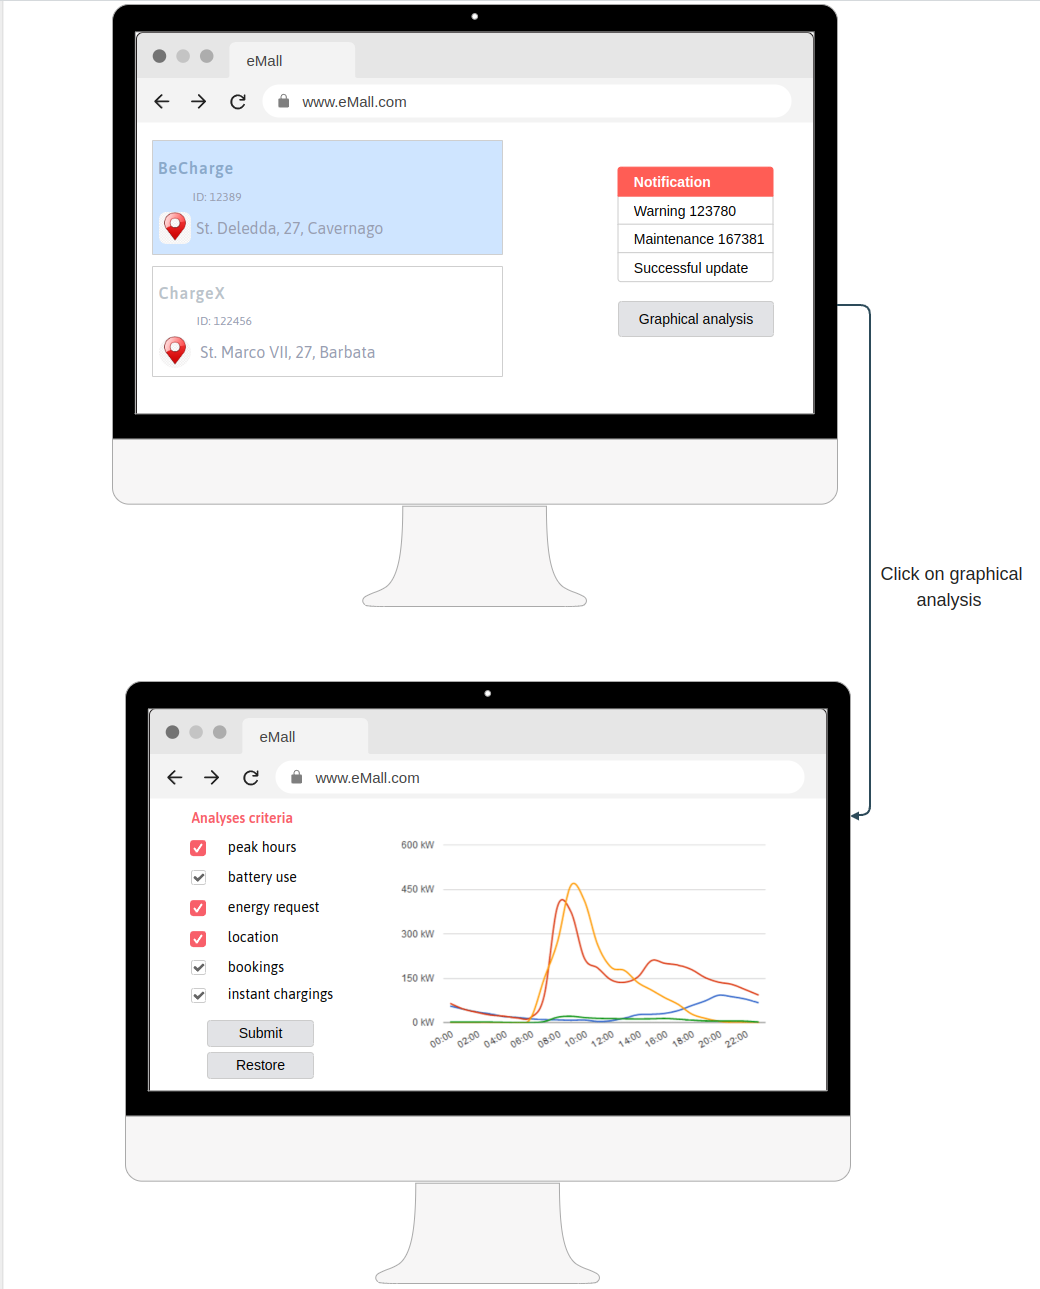
\includegraphics[trim={0.5cm 0cm 0cm 0.2cm},clip,width=0.75\textwidth]{Images/cp3/stationAnalysis.png}
    \caption{UI for analysing the stations}
\end{figure}
From the homepage, as explained before, the CPO can click the button 'Graphical analysis' and a new page is shown in which he has to select the criteria wanted for the analysis. Once submitted the choice, the eMall takes a few minutes to process the needed data and create a graphical view, that is shown reloading the page. In the reported UI we show an example of a graphical representation of the stations analyzed based on their location and on the energy request in order to identify the peak hours in which the service is used.  
\clearpage

\chapter{Requirements traceability}
\label{ch:chapter_four}%
\section{External Interface Requirements}
\label{sec:External Interface Requirements}%

\subsection{User Interfaces}
\label{sec:user interfaces}%
In this subsection we provide some mockups that show an example of some possible user interface, one for the mobile app which will be available to the users and one for the web app available to the businesses, that offer the charging service.

\paragraph{EVD interaction with the mobile app of the eMall}
The EVD needs to download the mobile app on his cellphone in order to interact with the eMall and take advantage of its functionalities. The Graphical User Interface (GUI) of the application is thought as an user-friendly interface, to facilitate everyone in using the service. In this first mockup we see the initial page of the system, shown to the user when opening the application.
\begin{figure}[H]
    \centering
    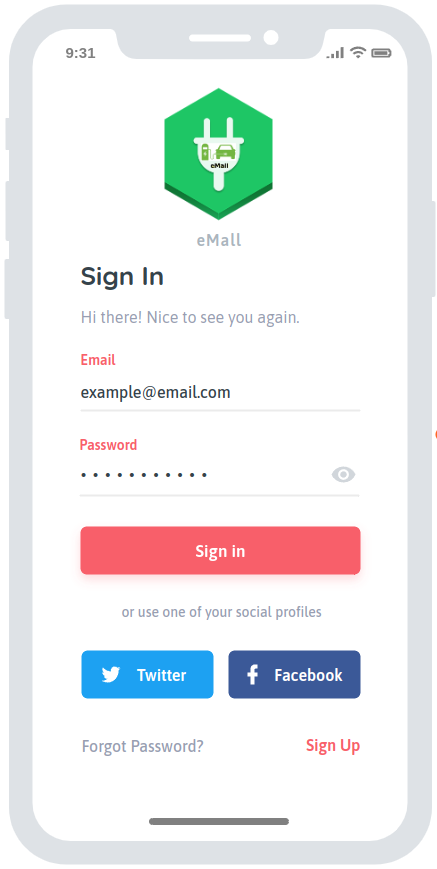
\includegraphics[scale=.3]{Images/cp3/signIn.png}
    \caption{Wireframe of the page that allows to log in from the eMma}
\end{figure}

In the following mockups we represent an example of the signing up procedure, showing the data required by the eMma in order to complete the creation of an account. 
\begin{figure}[H]
    \centering
    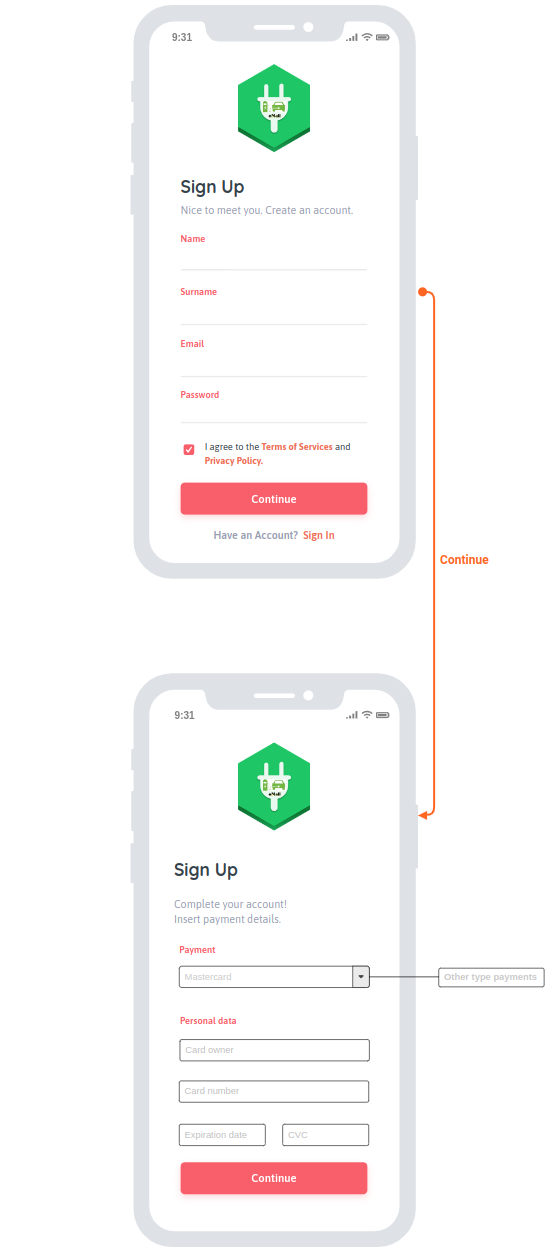
\includegraphics[scale=.45]{Images/cp3/signUp.png}
    \caption{Wireframe of the signing up process that allows to register from the eMma}
\end{figure}

\paragraph{CPO interaction with the managerial web app of the eMall}



\subsection{Hardware Interfaces}
\subsection{Software Interfaces}
\subsection{Communication Interfaces}

\section{Functional Requirements}
\label{sec:Functional Requirements}%

\section{Performance Requirements}
\label{sec:Performance Requirements}%

\section{Design Constraints}
\label{sec:Design Constraints}%

\subsection{Standards compliance}
\subsection{Hardware limitations}
\subsection{Any other constraint}

\section{Software System Attributes}
\label{sec:Software System Attributes}%

\subsection{Reliability}
\subsection{Availability}
\subsection{Security}
\subsection{Maintainability}
\subsection{Portability}


\chapter{Implementation, integration and test plan}
\label{ch:chapter_five}%

\chapter{Effort spent}
\label{ch:chapter_six}%
\label{sec:Effort spent}%
\begin{table}[h!]
    \centering
    \begin{tabular}{|l|c|}
     \hline
     \textbf{Activity} & \textbf{Time spent} \\
    \hline
    Organization & 5h \\
    \hline
    Understanding the problem & 10h \\
    \hline
    Introduction to the problem & 10h \\
    \hline
    Scenarios and overall description & 10h \\
    \hline
    Functional and non-functional requirements & 22h \\
    \hline
    Formal analysis using Alloy & h \\
    \hline
    Total time spent & h \\
    \hline
\end{tabular}
    \caption{The time Bianca Savoiu has spent working on this project}
    \label{tab:Assumptions}
\end{table}


\begin{table}[h!]
    \centering
    \begin{tabular}{|l|c|}
    \hline
     \textbf{Activity} & \textbf{Time spent} \\
    \hline
    Organization & 5h \\
    \hline
    Understanding the problem & 10h \\
    \hline
    Introduction to the problem & 10h \\
    \hline
    Scenarios and overall description & 8h \\
    \hline
    Functional and non-functional requirements & 12h \\
    \hline
    Formal analysis using Alloy & h \\
    \hline
    Total time spent & h \\
    \hline
\end{tabular}
    \caption{The time Fabio Lusha has spent working on this project}
    \label{tab:Assumptions}
\end{table}

%\chapter{References}
%\renewcommand{\bibname}{Whatever floats your boat}
\nocite{*}
%\bibliographystyle{plain}
\printbibliography[heading=bibnumbered, title={References}]
\label{ch:chapter_six}%

% LIST OF FIGURES
\listoffigures
 
% LIST OF TABLES
\listoftables
\cleardoublepage
\end{document}
